%% LyX 2.4.2.1 created this file.  For more info, see https://www.lyx.org/.
%% Do not edit unless you really know what you are doing.
\documentclass{article}
\usepackage[T1]{fontenc}
\usepackage[utf8]{inputenc}
\usepackage{color}
\usepackage{float}
\usepackage{varwidth}
\usepackage{amsmath}
\usepackage{graphicx}
\usepackage{geometry}
\geometry{verbose,tmargin=1in,bmargin=1in,lmargin=1in,rmargin=1in}

\makeatletter

%%%%%%%%%%%%%%%%%%%%%%%%%%%%%% LyX specific LaTeX commands.
\newcommand*\LyXZeroWidthSpace{\hspace{0pt}}
%% Because html converters don't know tabularnewline
\providecommand{\tabularnewline}{\\}
%% Variable width box for table cells
\newenvironment{cellvarwidth}[1][t]
    {\begin{varwidth}[#1]{\linewidth}}
    {\@finalstrut\@arstrutbox\end{varwidth}}

%%%%%%%%%%%%%%%%%%%%%%%%%%%%%% User specified LaTeX commands.
%\usepackage{epstopdf} % to include .eps graphics files with pdfLaTeX
\usepackage{flafter}   % Don't place floats before their definition
%\usepackage{topcapt}  % Define \topcation for placing captions above tables (not in gwTeX)

\usepackage{xurl}      % better URL setting, uses old url package

\usepackage{xcolor}
\definecolor{darkblue}{rgb}{0,0,0.4}
\usepackage[]{hyperref} % Generates all cross references
\hypersetup{            % Setting options for hyperref package
	breaklinks=true,    % break line with long hyperlinks
	colorlinks=true,    % coloured links
	linkcolor=blue,
	filecolor=magenta,
	urlcolor=darkblue,
	citecolor=blue,
	backref=page
} 

\usepackage{memhfixc}  % remove conflict between the memoir class & hyperref
\usepackage{pdfsync}   % enable tex source and pdf output syncronicity

\usepackage{memhfixc}  % remove conflict between the memoir class & hyperref
\usepackage{pdfsync}   % enable tex source and pdf output syncronicity

\usepackage{alltt}

% \usepackage{listings}
% \usepackage{xcolor}

% \lstdefinestyle{mystyle}{
%   language=Python,
%   numbers=left
% }

% Put lstset here, after lstdefinestyle
% \lstset{style=mystyle}

\makeatother

\usepackage[american]{babel}
\usepackage{listings}
\lstset{language=Python,
extendedchars=false,
frameround=fttt,
numbers=left,
% line numbers use none,
numberstyle={\tiny},
stepnumber=2,
% line numbers only every so many,
numbersep=9pt,
% how far line numbers from text?,
showspaces=false,
showstringspaces=false,
showtabs=false,
tab={\rightarrowfill},
basicstyle={\small},
keywordstyle={\color{blue}},
commentstyle={\color{green}},
stringstyle={\ttfamily \color{magenta}},
identifierstyle={\color{black}}}
\begin{document}

\title{Dispersion: the effects of aquifer heterogeneity\\
c o n c e p t}
\author{prof. dr.ir. T.N.Olsthoorn}
\date{2025-04-18}
\maketitle
\begin{center}
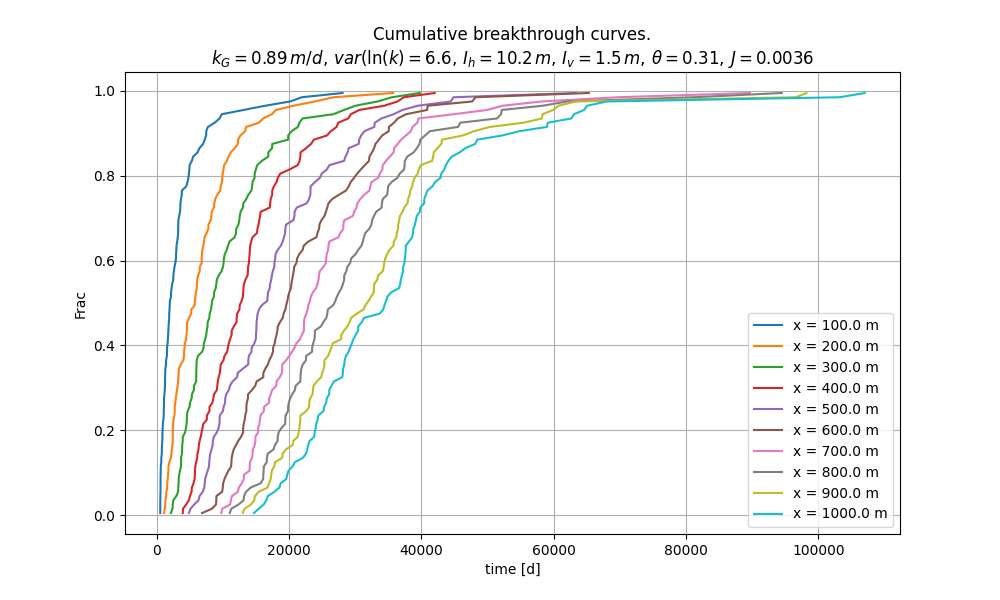
\includegraphics[width=0.7\textwidth]{/Users/Theo/GRWMODELS/python/mf6lab/Projects/Dispersion/cases/wimsaquif/images/cumulatives}
\par\end{center}

\tableofcontents{}

\section{Introduction}

According to \cite{Lange20,Lange22,Lange25} dispersion as we see
it through sampling an aquifer, is almost completely caused by groundwater
velocity variations on macro-scale and neither on velocity variations
at the pore-scale nor on molecular particle movement caused by diffusion.
Although pore-scale velocity differences always plays a role whenever
groundwater is flowing, and diffusion even when it's not flowing,
these two mechanisms are by many scholars believed to play such a
small role in most real-world situations, that they can often be neglected
when evaluating actual dispersion in the field or when modeling mass
transport with dispersion.

So what is dispersion as we see it? Dispersion can be defined based
on the gradual concentration increase, the reaching of a peak concentration
followed by the slow decrease of a consituent when a well or an observation
screen is frequently sampled. Dispersion can also be defined based
on the average concentration over the height of the aquifer sampled
by many vertically arranged small sampling screens or by sampling
a fully penetrating well. With the latter method, using more than
one well or series of sampling points at different spatial locations,
we may try to outline the extent of a so-called plume of pollutant
as it extents at a certain moment in time within the aquifer. We may
try to accomplish the same thing by sampling one or multiple wells
over time, taking into account the actual velocities of the groundwater,
which are oftentimes difficult to determine.

Dispersion has mostly been defined as a process similar to diffusion,
in that it is due to velocity differences at the pore-scale, which
cause diffusion-aided mixing between adjacent streamlines and thus
result in the observed spread of the pollutant both in the direction
of the flow as well as perpendicular to it. In this traditional Fickian
or Gaussian theory the spreading behaves as if it was driven purely
by concentration gradients. In fact, without diffusion, at least,
theoretically, a pollutant should not spread perpendicular to the
streamlines in all cases where streamlines cannot cross each other.
Streamlines can only cross each other in 3D space, and, therefore,
such advection mechanisms cannot explain spreading of a pollutant
perpendicular to streamlines in 2D space. Nevertheless streamlines
can cross each other in 3D space (e.g. in aquifers with hoirzontal
layers having main horizontal conductivity axes in different directions
\cite{HemBak04}, \cite{Jankovic03,Jankovic10}). This eventually
reduces the value of 2D dispersion analyses in a fundamental way as
it remains impossible to determined the 3D impact happening in reality
using a 2D simulation.

However, major velocity differences occur on macro scale, caused by
differences of the hydraulic conductivity and or porosity on the scale
of the sedimentation processes that originally formed the aquifer.
Notice that we only consider aquifers consisting of sediments, that
is, aquifers constructed of layers of particles of different sizes,
as show up in borelogs and cross sections alike. These processes have
built up the aquifer over large spans of geologic time, in layers,
formed in different energetic environments, i.e. by water that carried
different amounts of particles the size of which varied depending
on the geologic and climatic circumstances. These circumstances have
liklely largely varied over the tens of thousands to millions of years,
during which the aquifer was formed. Retracting seas during ice ages
and rising land cause larger gradients of the earth's surface, due
to which erosion increases and more and coarser sediments are laid
out over extended areas, generally by wide braided rivers. Their sediments
cause coarse-grained inclusions, which are detected in our current-day
aquifers. During warmer, more vegetated eras, with higher ocean levels,
rivers carry less and finer sediments, While meandering they cut into
previously deposited sediment layers to form their characteristic
patterns we now observe in cross sections. During cold windy periods
with tundras as well as in dry deserts, large-scale areal transport
and deposition of fine particles have formed often vast regions with
moving dunes, which now show up in cross sections as often thick layers
of overlapping sublayers of fine material. They are characterized
by their upward curved patterns that witness the original horizonal
progress of the dune-type deposits. Extended clay layers are generally
caused by sea transgressions when climate warmed up or land sank.
Or they were deposited by rivers that broke through their banks creating
extended flood areas with little energy, which allowed fine particles
to settle and to form river-clay deposits. We oftentimes witness all
such previously active processes play out in the bore-hole profile
or in natural or our own man-made cross sections. Looking at such
profiles, we are watching how a vast number of geological processes
has played out over hundreds of thousands to millions of years to
form the aquifer at hand. No wonder the details of the flow of groundwater
through an aquifer is complicated. When dealing with the groundwater
head in an aquifer or at what rate we can extract water from it by
a well, things are far less complicated due to natural averaging of
the head between layers and the integration of the flow towards a
well screen over all layers that intersect it. However, if we study
the spread of pollutants within an aquifer, the details of the structure
of the aquifer do matter. And it's obvious that the extremely wide
variation of the conductivity within the aquifer, caused by the mentioned
varyity of sedimentation (and local erosion) processes, determine
the spread of a pollutant more than velocity variations at the porescale.
As far as diffusion is concerned, it's important over the long run
in stagnant situations and to allow consituents to jump between parallel
stream lines. But on local scales and relative short, say sub-century
time scales it tends to be of little importance.

While an aquifer tends to be built up over time by repeated fining-up
sediment sequences, it is the braided river's coarse material deposition
during cold periods that intersects such layered sequences and created
inclusions with often sharply distinct hydraulic conductivities. To
a somewhat lesser extent, we find ,,inclusions'' (often called facies)
caused by meandering rivers that cut into older layers while eroding
their outer bends and at the same time deposing fresh material at
their inner bends. This way, meandering rivers create their charactistic
particle-band patterns in cross sections with their associated conductivity
patterns. But we also encounter existing sediment packages that were
disturbed, pushed up, shifted and partly or toally turned over by
the heavy load of progressing land ice. When retracting and after
melting, the deep valley space that was left over, was subsequently
filled up by both erosion material from the pushed-up ridges and filled
by fine material, especially caused by subsequent sea water rise.
Of course, much more can be, and perhaps should be said about the
characterisics of the cross sections we encounter in the field. Studying
and describing them has been the focus of geologists and especially
sedimentologists throughout the world over a long time. However using
their discriptions to accurately model the hydrogeneous conductivity
field remains a challenge and is mostly not universily successful
to say the least.

The fundamental consequence of attributing all ,,disperision'' to
spatial conductivity variation in facies and inclusions, i.e. by neglecting
pore- and grain-scale processes, is, that, in fact, no mixing can
occur in the subsurface because it implies that every particle will
stick to its own original streamline over its entire underground life.
This would even be true when the streamline changes over time as a
result of altered boundary conditions. Hence, with this asusmption,
all dispersion, i.e. mixing, occursat the extraction point, where
the extracted water is mixed in the screen or the well when pumping
or just sampling it. Or, the water is mixed in the computer when we
digitally mix the extracted water along the vertical at some point
in the aquifer. There may be differences between physical and digital
mixing, though. For instance, the mixing in a well screen depends
on the flow from each layer that intersects the assumed fully penetrating
screen. This makes the layers with the highest conductivities dominant,
as we often see when measuring the inflow to a well screen along its
length. To get the right comparison, in the computer we must also
take the afflux at each elevation along the well screen into consideration,
which is not difficult to do. We can also do this over time. But in
fact, when mixing the water vertically at a given point in the aquifer
and a given point in time, we always mix water from layers with zero
consituant concentration with water from layers with non-zero constituent
concentration. And, under the assumption that only advection is active,
a streamline either has exacly the same concentration it was given
at the point of release after passing the point of none. This is a
consequence of the assumption of zero mixing within the aquifer, which
is what happens as particles stick to their streamline and pore-size
processes are ignored. Hence, each streamline either carries a particle
of the constituent or none at the moment and point of sampling.

When simulating discrete particle transport in the computer, the probability
of hitting any particle at any streamline at the well exactly at the
time of sampling may be vanishingly small. Therefore, we have to sample
over a given amount of time, to capture at least some particles. Afterwards
we integrate over time to get the cumulative probability distribution.
Or rather considering an initially sharp front, we simply count the
streamlines whose front particle has passed the observation point,
sort these times and construct the cumulative breakthrough curve for
this .

How then can we define dispersion when we consider it to be caused
by advection through the heterogeneous aquifer alone? One way to do
it, is by recording the particles that were initially released at
one location and time, as they pass some point downstream. When the
particles were initially distributed vertically in such a way that
each of them represents the same fraction of water, while the total
number of particles make up the entire groundwater flow, then we can
construct the cumulative distribution of particles passing the observation
location. The shape of this distribution represents the statistics
of the advection-dispersion process in its entirety, and its derivative
represents the density distribution, allowing for further statistical
analysis and statistical generalization.

When we only take advection into account, it is fundamentally impossible
to determine the dispersion after releasing particles at a single
point and time, i.e. due to a concentration pulse. This impossibility
is due to a sudden release of a given number of particles at a single
point in the aquifer at a given point in time. This is so, because
if this point source is theoretically a single point in the aquifer,
then all particles would be on the same stream line and stick to it
and would always travel at the same speed. Hence, no dispersion would
ever occur within this framework. The fact alone that a point source
does generate a growing plume in reality, implies that this concept
of pure advection, may have its merits, but also has its limits.

No one dan ignore that diffusion acts in groundwater, as it is caused
by molecular movement, which is always present. The spread $\sigma$
of an initial concentration pulse, or of an initially straight concentration
front, is defined by the standard deviation $\sigma=\sqrt{2Dt}$ with
$D$ {[}L$^{2}$/T{]} the molecular diffusion coefficient. With a
value of $D\approx2\times10^{-9}$ {[}m$^{2}$/d{]}, we have $\sigma\approx0.25$
m in one year. This is not nothing. It spread will defnitely does
cause particles to step over to adjacent streamlines. In 100 years
$\sigma\approx2.5$ m and in 10000 years $\sigma\approx25$ m. The
latter is of the scale of the vertical exent of the aquifer itself.
Hence, on the long run diffusion as a mechanism to spread out pollutants
perpendicularly to the streamlines cannot be ignored and will limit
the value of the pure advection approach to tens of years rather than
hundreds or even thousands of years.

\section{Analysis of advection-dominated dispersion using particle tracking
in heterogeneous aquifers in 2D vertical cross sections}

Assuming that dispersion is caused by macroscale velocity variations
due to the aquifer's heterogeneous conductivity field, we can analyze
it by means of particle tracking. In order to include diffusion (but
still ignoring porescale velocity variations) we would have to include
mass transport with diffusion, which is outside our current scope.

Even realizing its limits, we will stick with a vertial, i.e. 2D cross
section of uniform height modeled with finite differences using a
rectangular mesh with sub layers of equal height. The conductivity
of each cell may be unique, and the vertical and horizontal conductivities
may be different. Furthermore, also the porosity in each cell may
be chosen to be unique. However, the variations of the porosity in
a real aquifer tend to be small, even negligible compared to the variations
in hydraulic conductivity. For this reason, without loss of generality,
we will use a constant porosity of around 35\% throughout our analysis.

The boundary conditions of the modeled cross section are a fixed but
different head at both ends. This would yield a uniform flow field
when the aquifer were homogeneous. However, due to its heterogeneity,
the flow field is far from homogeneous and will be determined by a
steady-state computation with Modflow. The results allow us to visualize
not only the lines of constant head, but also the lines of constant
values of the stream function. The stream function allows us to determine
uniquely the flow density and the flow direction at any point in the
aquifer, even without particle tracking. The stream function permits
us to detemrine the elevation of the release points of the particles
such that each particle represents the same amount of discharge, which
will guarantee keeping the mass balance also with particle tracking.

Particle tracking is done with Modpath7. Modpath guarantees that the
governing differential equation of the discharge is fullfilled at
every point within every cell of the model. This implies that, although
the model is only a limited representation of the actual aquifer,
particle tracking the Modpath way does guarantee proper distribution
of the particles throughout the aquifer while maintaining the mass
balance at any point as well as in the aquifer as a whole.

The procedure to follow is to first generate a conductivity field.
Then use Modflow to compute the flow field in the aquifer, with heads
and cell-by-cell discharges. This is ollows by the computation of
the stream function using the flow across the right face of the cells
that were computed by Modflow. The next step is to place particles
along a vertical in the aquifer at elevations obtained from the stream
function, such that each particle represents the same amount of discharge
along this vertical. After releasing the particles they are tracked
with Modpath. Following step is to take the computed pathline file
and for each particle compute when exactly it passed a set of given
points in the aquifer. Finally we determine the cumulative breakthrough
curve for each of these locations. These breakthrough curves represent
the cumulative probability density function of the dispersion between
the release point and the observation point, they capture the characteristic
of the dispersion processes active between the two points. By using
more points, the development of the cumulative density function over
time or, rather distance, can be studied. These cumulative probability
density functions can be converted into breakthrough histograms to
unveil the underlying probability density functions. Both cumulative
breakthrough curves and the histograms contain the same information.

\section{Literature discussion}

A vast number of papers has been written on subsurface transport of
pollutants (Gelhar, Sudicky ...). This mainly started in the 1980s
after it became obvious that hunderds of thousands of waste sites
were and have been polluting groundwater and groundwater and as avaluable
resource for drinking water and public concern skurocketed. The study
of the subsurface displacement and spreading proved difficult due
to the heterogeneity of the subsurace and the interaction between
pollutants and subsurface material. The studies were plagued by lack
of understanding the complexity of the conductivity field that caused
preferential flow paths and the mixing processes known as dispersion
as well as the role of diffusion in it. The Fickian of Gaussion theory
that look so nice on paper, or in math, was time and again challenged
in practice, where samples showed that reality adn theory more often
than not did not match. Hence long time studies were underrtaken with
large-scale and repeated tracer tests to better capture and learn
to predict what happens in practice. The Borden en Made studies, both
done over 25 years with millions invested in exploring the subsurface
structure and sampling the groundwater in great detail were carried
out, but in the end did not totally solve our lack of insight and
modeling capabilities to correctly predict development of pollution
plumes in those and other circumstances.

Sudicky (1986) carefully studied the Borden experiment after others,
like Dagan and Gelhar went before him. Hij gives a cross section in
both the longidudinal and perpendicular direction to the grounwater
flow. His paper is more or less a summarizing evaluation of the work
that was done at Borden. Sudicky considers the flow as fundamentally
3D and finishes with a summary worth citing from it.

Zheng et al. (2011) provide a review and overview of over 25 years
of research and lessons learned at the Macrodispersion Experiment
(MADE) site, located at the Columbus Air Force Base in Mississippi.
The site has been instrumental in advancing the understanding of solute
transport in highly heterogeneous aquifers. The authors conclude:
,,In spite of tremendous effort and progress over the past three
decades, our ability to predict solute transport processes in highly
heterogeneous media remains very limited''. They show to expect a
lot from future field measurements in a comprehensive suite and carefully
designed in a tightly integrated fashion. However, it's doubtful if
these new studies will be ever perfomed, given the effort and cost
already spent before. It seems that the existing data for the Made
and Borden will be revisited in new research for a long time into
the future. The authors stress that future work should focus on mapping
the hydraulic conductivity distribution and the resulting preferential
pathways far beyond what is currently possible given the existing
measurement techniques. With this disclamier the authors seem to admit
that the problem to fully understand subsurface transport will remain
essentially unsolved for a long time in the future.

Gorelick has essentially introduced the dual domain theory and model
to better capture the observed dispersion at the very heterogeneous
Made site (\cite{Zheng11}). The dual domain was then included in
several groundwater transport codes. like MT3SM. The dual domain just
discerns between a mobile phase and an immobile phase, with kinetic
exchange process between them. It has been quite succesful in Made
as is shown in figure 9 in \cite{Zheng11}. It thus seems that a dual
domain can compensate for the failure to accurately capture the hydraulic
conductiviy field to mimic the transport behavior with preferential
flow paths. However, it may well be that the dual-domain model functions
well for the wrong reasons by being able to produce a subsurface mass
transport that mimics the measurements even if in reality there are
not two domains but there is just a very heterogeneous conductivity
field. The authors seem to admit this in their introduction stating
that ,,results from field investigations and modeling analyses suggest
that connected networks of small-scale preferential flow paths and
relative flow barriers exert dominant control on solute transport
processes.'' Thse connected networks are fundamentaly different from
the adsorption process that is modeled by the dual domain seems to
make no sense to model consituents that do not sorb like chloride,
bromide or tritium. \cite{Fiori13} show that indeed, it is possible
to get similar outcomes with a heterogeneous conductivity field without
a dual domain with sorption.

Two years after this review paper that should have said it all was
picked up by \cite{Fiori13}. They continued the dicussion and tried
to model the observed plume dispersion at the Made site. To better
tackle the large asymmetry of the pollution plume not described by
traditional advection-dispersion models, they propose a multi-indicator
model (MIM). With it \cite{Fiori13} essentially subdivide the aquifer
into blocks of different independent conductivity drawn from a lognormal
distribution. The dispersion generated by the flow of particles through
their heterogenious model was the resdult of advection alone. They
found that this simple advection model could describe the development
of the observed plume ,,remarkebly well''. In their section 3, the
authors explicitly motivate their claim that advection is the only
process that matters at the Made site. With the few parameters given
in their table 1, and used below in this report, their MIM model was
capable of mimicking the measured bromide distribution sampled at
6 points of time, but only reasonably. Nevertheless, their MIM model
did demonstrate that the observed dispersion can be explained just
by the flow as it is distored by the heterogeneity of the conductivity
field in the aquifer, even without considering any other processes.
The results of this advection-dominated model show the charateristic
that proved impossible to model with traditional advecton-dispersion
models, which is the large asymmetry (long tail) of the plume development
in the subsurface.

The more homogeneous the conductivity field of the aquifer is, the
less dominant is the spread of particles caused by advection and the
more important diffusion and pore-scale velocity differences will
be. Even then these low-scale velocity differences will dominate diffusion,
at least in the flow direction. For instance, \cite{Jensen93} show
that, even though their Danish aquifer is very homogeneous, the derived
longitudinal dispersivity was 500 times larger than the transvese
dispersivity and 1000 times larger than the vertical transverse dispersivity.
From this, we may conclude that velocity variations caused by local
small scale conductivity variations are likely the cause of the large
contrast between the vertical and transverse dispersivities. \cite{Jensen93}
proved this by showing that inceasing refinement of their model better
mimicked the small-scale statistics of the aquifer.

\cite{Jankovic06} show that, even though macrodispersion can be described
by velocity variations caused by the conductivity field, and result
in largely asymmetric plume shapes with a short front and a long tail,
the bulk of the plume can still be described by a Gaussian model with
an equivalent mean velocity and a longitudal dispersivity. This does
not work for the long tail, but the tail will be of far less importance
in practice as it only holds a small fraction of the total mass of
the pollutant. Only when the aquifer tends to homogeneity, the Gaussian
model will also better predict the plume's tail behavior. \cite{Jankovic06}
further conclued from their work, that for very inhomogeneous aquifers,
the plume behavior does not approach Gaussian / Fickian behavior even
for very long travel distances.

\begin{figure}[H]
\centering
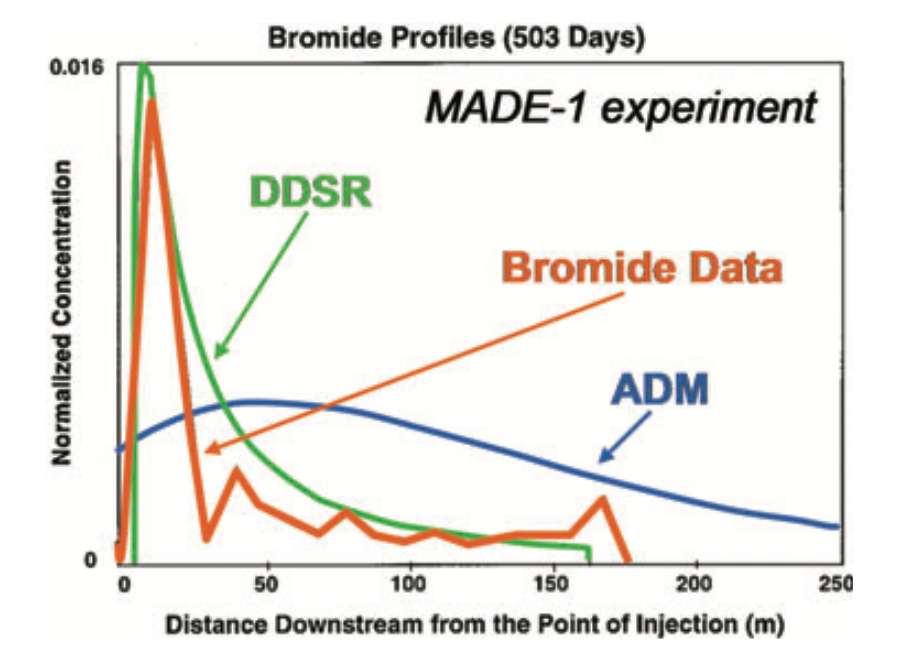
\includegraphics[width=0.5\textwidth]{../images/zheng_ea_2011_fig9}

\caption{\label{fig:Comparison-models-Made}Comparison of the modelled and
measured bromide plume extent at the Made site. ADM stands for classical
Advection-Dispersion-Mass transfor model, DDSR stands for Dual-Domain
Mass Transform Model. The graph clearly shows the rapid progress of
a small part of the water while the bulk remain near the source. The
intepretation depends on whether the flow rate hat the sampling elevations
was included in the analysis. This is probably not the case.}
\end{figure}


\section{Cross sections}

\subsection{Introduction}

A fundamental problem, perhaps the most fundamental one, is that the
flow in a 2D cross section misses the thrid dimension. The problem
is not that some cross section is bended to follow the curves of a
projected streamline, nor that the cross section represents an axially
symmetric situation. The essence is that a plain crosss section does
not have flow components perpendicular to it. In theory a 2D section
does not require flow components perpendicular to it; in practic,
this is never fully the case. Wherever the flow and the spread of
particles is determined by inhomogeneities, or, in other words, by
the heterogeneous conductivity field, due to which the flow direction
continuously deviates from the average flow direction in the cross
section, one can then be certain that in reality such deviations also
occur perpendicular to the 2D plane of the cross section. The inhomogeneities
of the real world are never limited to the plane of the cross section,
they are just as strong perpendiular to it. \cite{HemBak04} and others
have shown, that exactly this 3rd component of the groundwater velocity
makes that stroomlines can cross each other, and thus cause dispersion,
what they never can in a 2D situation. The analysis of the flow in
a flat cross section falls fundamentally short to discribe the full
mixing process in an aquifer characterized by its heterogeneous conductivty
field in all its 3 dimensions. The paper of \cite{HemBak04} triggered
3D thinking and made crystal clear the likelihood, or perhaps even
the certainty, that a 3D inhomogeneous conductivity field will let
streamlines cross each other all the time and everywhere, and thus
cause mixing at a scale much larger than that at which molecular diffusion
or pore-scale velocity differences play.

And of course particles (molecules) will jump between adjacent streamlines
all the time, which, combined by the turnover of streamlines described
above, triggers transversal spreading at a rate that far exceeds that
of molecular diffusion. Molecular diffusion tends to be slow and becomes
increalingly slower over time as expressed by the formula for the
grow of the standard deviation of an initially sharp front, i.e. $\sigma=\sqrt{2Dt}$.
However, in a porous medium like an aquifer, in which the velocity
varies perpendicular to the stream lines everywhere, the concentration
gradient perpendicular to the streamlines is kept much sharper. This
is a consequence of the washing process associated with particles
on adjacent streamlines having different volocities. This washing
process cause molecular spreading to be larger than in the theory
valid voor a stagnant groundwater.

Finally, it is virtually impossible to determine particle concentration
at distinct points in the aquifer. We do not get around the fact what
we will always mix water from different streamlines when sampling,
no matter how we do this. This is true for even the smallest sampling
screen, for a sampling well and for measuring concentration using
some physical device, for instance by measuring electric conductivity
or tracer color. If we consider advection to be the dominant or even
the only relevant process taking place in the aquifer, then mixing
will only take place at the moment we sample or extract. The best
we can hope for is the sampling of the passage of a complete front.

To this we must add the the difference between sampling is situ without
disturbing flow, for instance by a sounding device, or by extracting
using for instance a well. Both methods will often given completely
different results as the extraction method mixes the incoming water
in proportions proportional to the conductivity along the screen,
with some parts yielding most and other parts yielding least water,
while sampling in situ measures without considering the amount of
flow that its elevation. Mixing these sampling methods can lead to
misinterpretations

In conclusion if we ever want to model groundwater mixing appropriately,
we must consider 3D velocity components, even when dealing with flat
cross sections. When sampling we must realize the mixing we cause
or not cause depending on the sampling method as the results may be
completely different. 

In the analysis for this work, we will at least initially focus on
the flow in vertical cross sections without any flow perpendicular
to them and should be aware of its limitations.

\subsection{Generating cross sections}

For any analysis we need a conductivity field first. There are many
ways to generate cross sections. One manner is to do this based on
a colored picture, by sampling the pixel colors, clustering these
colors, and then assigning distinct conductivities to each of them.
Although doable, and allowing many pictured cross sections to be used
in this way, the resulting sections will always be artificial as no
single hand-made image of a cross section can ever grab, even nearly,
the real-world conductivity variations that are present in reality.
These cross-section pictures have too few colors, and on top of this,
the colors tend to picture perceived facies or formations rather than
conductivities.

Cross sections may also be obtained from websites that provide them
based on borelogs and other physical logs, cores etcetera. Such geological
sections are exactly those meant above. However, sites such as Dinoloket.nl
provides a full 3D database of the lilelihood of the occurence of
a set of materials (sand, clay etc.) for blocks (voxels) of some 100x100x0.5
m across a large part of the Netehrlands. It is straightforward to
extract colored cross sections form this website and use them in the
way described above. However, these data are also very limited in
that the number of voxels is much larger than the resolution of the
underlying data, so that they do not represent reality, but instead,
the probability of the occurrence of given materials, which can then
be associated with conductivities. If we associate one conductivity
with each voxel, then the result is likely too coarse to accurately
simulate subsurface transport as caused by the more local heterogeneous
conductivity field.

One can digitally generate borelholes by using transistion probabilities
between adjacent materials as obtained from borehole sampling. The
resulting borehole is clearly artificial, but it will at least have
some statistical properties similar to that of the real borehole.
The problem then becomes how to link manyin this way created boreholes
together into a single cross section. Simple interpolation will not
be enough as it then ignores the horizontal transitions or at least
the scale of them. And it is not clear how to solve this issue without
external information, which, in fact, cannot come from boreholes drilled
at mutual distances in the order of hundreds to thousands of meters.
Such information could come from the study of existing real-world
cross sections for similar sedimentological environments. It is likely
that the number of real-world cross sections that actually match the
sedimentologial environment in the subsurface in which we drill our
boreholes, is far too small to yield accurate data.

From such cross sections rather than from individual boreholes that
are too far apart, we can extract the statistics of the grainsizes
or even the hydraulic conductivity in the horizontal and vertical
direction by constructing semi-variograms. Then use these to statistically
generate individual cross sections, also know as realisations, which
at least have this same statistical properties as the real cross section.
The problem is, that each realization is different and no one will
mimic the actual field situation accurately. The only thing we can
then do, is generate a large number of such realisations and study
the properties for the ensemble, the results of which are always statistical
themselves.

Finally, we can just generate our 2D cross sections, or even complete
3D conductivity fields digitally be sampling from conductivity distributions
in some way (\cite{Fiori13}) or by placing distinct heterogeneities
in a 2D or 3D field (\cite{Jankovic03,Jankovic06,Jankovic10}), of
which the link to reality will remain unanswered. 

\section{Cross section according to De Lange}

\nocite{Lange20,Lange22,Lange25} in his papers, takes an approach
that is similar to that of \cite{Fiori13} et al. He divides his vertical
cross sections for the sake of dispersion simulation into blocks,
which he calls domains. These blocks have a background conductivity
with one embedded elongated facies with a conductivity that is largely
distinct from the block's background value. The entire dispersion
process takes place inside the block. To simulate a long travel distance,
many alike blocks are placed next to each other and on top of each
other, thus filling the entire space of the vertical cross section.

We can generate such cross section by creating a conductivity field
that mimics De Lange's multiple block aquifer.

\subsection{Cross section between De Lange and \cite{Fiori13}}

We can also just fill the entire cross section with blocks of the
same size, each of which has it's own distinct conductivity drawn
from a statistical, i.e. lognormal distribution. The cross section
will then be similar to the model domain used by \cite{Fiori13} at
al.

\subsection{More elaborate cross sections}

A next step to more realism is to make sure that not only the probability
of encountering certain conductivity values matches that in the real
aquifer, while also honouring their spatial covariance or their horizontal
and vertical transition probability. This should better mimic the
extent of the heterogeneities at the scale of the layers in the aquifer
and the horizontal structure that we observe in actual geological
cross sections. In fact, doing this, will satisfy the statistics of
the real cross section as while keeping it's character determined
by adjacent distinct facies, but the aquifer may look completely different
that the real one. It's just a computation object required by our
model.

\subsection{Going fully geostatistical}

Going fully geostatistical would be a final stap towards more realistic
simulations. However, simple semi-variograms of the distribution of
conductivities will not be enough; generating cross sections from
it would smear out the distinct boundaries between facies. Hence,
going fully geostatistical will require advanced geostatistical methods
to allow honouring all features that we observe in real-world cross
sections.

\subsection{Finally still lacking the third dimension}

Even if we go fully geostastical to maximize the match between our
digital and real-world cross section, we still miss the third dimension,
which may prove essential for mixing by the likely ubiquitous 3D cross-over
of streamlines with associated particle exchange. This simply implies
that we either include the third dimenension in our cross section
or we mimic its effects by introducing some vertical mixing process
that mimics it, like vertical dispersion. It's importance may vary
though, but totally excluding it may prove wrong, especially in high-conductance
zones.

\subsection{Choice of the cross section type}

Because high-conductive facies of some horizontal extent seem to matter
most for the observed pollutant breakthorugh curves, our cross section
must reflect this. There are different ways to generate sections with
such properties. The one we adopt here is inspired by \cite{Fiori13},
\cite{Lange20} and the sedimentological origin of them as explained
in \cite{Coe03}.

A rectangular array of conductivity zones is created. Then a cell
in the array is arbitrarily chosen to center the next zone. The height
and width of the zone are then chosen to label the area of the overal
conductivity array. This is done until all cells of the conductivity
array have been labeled. As a last step, the conductivties are randomly
selected from a log-normal distribution and associated with each of
the labels to generate the final conductivity field.

The conductivity field was generated using the data of \cite{Fiori13},
table 1.
\begin{description}
\item [{$K_{G}=8.9\times10^{-6}$}] Geometric mean of $K$ {[}m/s{]}
\item [{$\sigma_{y}^{2}=6.6$}] Logconductivity variance
\item [{$I=10.2\,m$}] Horizontal integration scale (range of the semi-variogram
of $k_{k}$)
\item [{$I_{v}=1.5\,m$}] Vertical intgration scale (range of the semi-variogram
of $k_{v}$)
\item [{$\theta=0.31$}] Porosity
\item [{$J=0.0036$}] Mean head gradient
\end{description}
I did not use the parameters $I$ and $I_{v}$ directly.

\subsection{\label{subsec:Made-cross-section}Made cross section as applied by
Fiori at al (2012)}

Because of their success, we will mimic the the consturction of cross
sections used by \cite{Fiori13} in their MIM (multi-indicator) model
to simulate plume break-through at the Made site. These sections consists
of cubic blocks of equal size, equal to $2R$. 

$Y=ln\left(K\right)$ is normal with $mean(Y)=\ln\left(K_{G}\right)$
and variance $\sigma_{Y}^{2}$ and of stationary symmetric autocorrelation
$\rho\left(r^{'}\right)$ where $r'=\sqrt{\left(\frac{r_{x}^{2}+r_{y}^{2}}{I^{2}}+\frac{r_{z}^{2}}{I_{v}^{2}}\right)}$

The conductivity field in figure \ref{fig:mim-kfield} has been generated
as an exponential random field according to the parameters used by
\cite{Fiori13}.

\[
C_{h}=C_{0}\left(1-e^{-\frac{h}{I_{h}}}\right);\,\,\,\,C_{v}=C_{0}\left(1-e^{-\frac{h}{I_{v}}}\right)
\]
These parameters are in the header of the figure. The zones all have
the same width, equal to $2I_{h}=21$m. The field was first generated
with gstools using an exponetial model with lengths equals to $I_{h}$
and $I_{v}$ using the values for the mean conductivity and the variance
of its logrithm as given in the figure \ref{fig:mim-kfield}. Next
the section was divided into blocks of width $2I_{h}$ and the conductiviy
value generated at its cente was attribured to the entire block. The
blocks on overlying layers are shifted relative to each other as was
done by \cite{Fiori13}. 

The $k$-field was then used in Modflow to compute the heads and flows
with fixed-head boundaries at both ends such that the mean head gradient
was $J=0.0036$. The Modflow results permit computing the stream function,
which is given in figure \ref{fig:stream-function}. No particle tracking
is needed for that. The stream lines, which are the contour lines
of the stream function, clearly show how the particles flow up and
down through the aquifer as caused by the heterogeneous conductiviy
field. From these vertical components it should become immediately
clear that there must also be components perpendicular to the cross
section in real-world circumstances, which are neglected here but
could be incorporated with a 3D model generated in the same way.

Figure \ref{fig:mim-paths} shows the pathlines as tracked by Modpath.
100 particles were released but only every 5th particle path is shown
for clarity. The release elevations based on the stream function,
are such that each particle represents the same amount of flow. The
pathline pattern matches perfectly that of the streamlines, as they
should in a steady-state situation. The heads are not shown here,
but they are shown in figure \ref{fig:stream-function}.

Figure \ref{fig:mim-cum-t} shows the computed cumulative breakthrough
curves at intervals of 100 m along the cross section. The times are
quite long, which is due to the length of the section and the enforced
gradient $J=0.0036$. Notice the long tails for the greater $x$-values.
Long tails are expected whenever the mass transport is essentially
caused by advection through an aquifer that is heterogeneous on scales
that are substantial with respect to the cross section. The size of
the heterogeneities of $2I_{h}=21$ m in this cross section can be
observed in figure \ref{fig:mim-kfield}.

Finally, we compute the histograms from the obtained cumulative breakthrough
curves. These overlapping histograms are shown in figure \ref{fig:mim-hist_t}.
The histrogram for $x=1000$ m clearly shows the asymmetry of the
density curve with its steep front and long tail, a phenomenon that
is characteristic for advection-dominated transport through a hegerogeneous
subsurface. To better analyze the outcome, the breakthrough times
curves have been fitted by the logrnomal distribution as shown in
figure \ref{fig:mim-BT_t}. The lognormal distribution fits very well.
Note that due to the skewness of the lognormal distribution, we have
$t_{mode}<t_{median}<t_{mean}$, the values of which are also indicated
in the figure. Instead of using the usual quantiles (0.05, ... 0.95
of the cdf) to indicate the bulk and outliers, we used 0.2, 0.5, 1.0,
2.0 and 5.0 the $t_{mode}-t_{0}$ as more informative values. The
pdfs are shown in the bottom figure and clearly demonstrate the skewness
of the break-throughtimes.

Figure \ref{fig:mim-BT-x} shows the position of the particles at
given observation times. These particle position were ordered and
fitted by the lognormal distribution, of which the cdf is shown together
with the outcomes of the simulation. The fit is less good than that
for the break-through times. The obvious reason for this is that for
the times, every particle has passsed the entire 1000 m length of
the model, where for the postioins of any given observation times
this is at all the case. Therefore, particles that traveled little
at a given time, have seen only a small part of the model's heterogeneity
and are thus subject to more randomness. The latter may only be solved
by repeated realizations and taking the ensemble at the end. The graphs
with the particle positions seem to more resemble the normal distribution
than those for the break-through times. However, this may especially
be the case for larger observation times. The graphs with the particle
positions also make clear, that a portion of th particles hardly moves
at all, which is indicative of tail formation. One is tempted to compare
the pdf with the particle position with the data for the Made site
as shown in figure \ref{fig:Comparison-models-Made}. There the mode
at $t=503$ d was at about 15 m from the source; in figure \ref{fig:mim-BT-x}
bottom at $t=600$ d it's at about 20 days, which is not too different.
Note that in this model the same aquifer and gradient values were
used as published for the test at the made site (\cite{Fiori13}).
All in all, I don't see that the result by \cite{Fiori13} is too
convincing as a travel distance of the mode of 15 m is small with
respect of their fixed box size of about 20 m, and therefore, really
small with respect to the size of the heterogeneities in their model,
implying that chance may play a big role at these outcomes.

\begin{figure}[H]
\centering
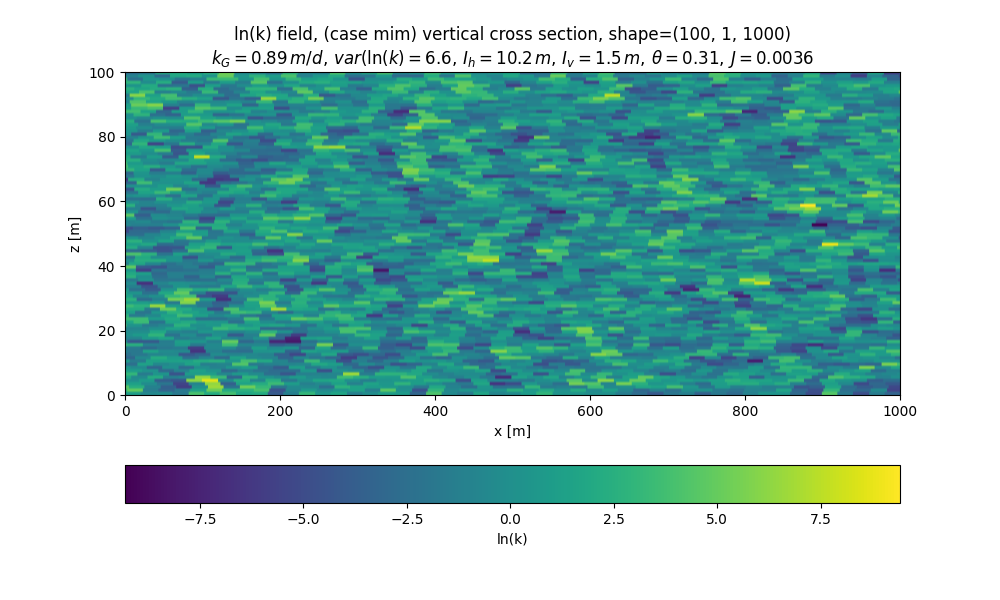
\includegraphics[width=0.8\textwidth]{/Users/Theo/GRWMODELS/python/mf6lab/Projects/Dispersion/cases/wimsaquif/images/kfield_mim}

\caption{\label{fig:mim-kfield}log-$K$-field, like in \cite{Fiori13} with
the same parameters (see header)}
\end{figure}

\begin{figure}[H]
\centering
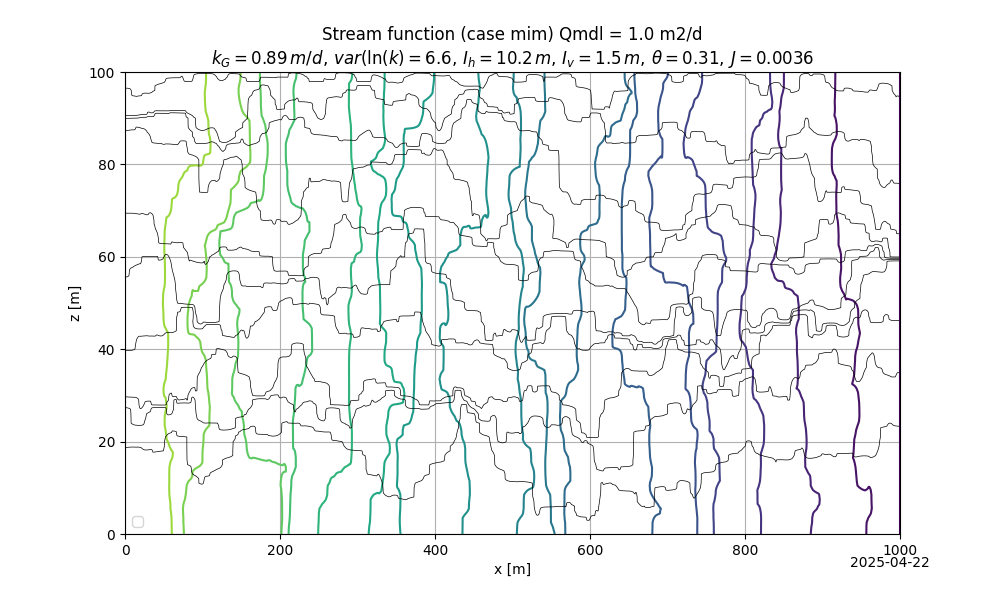
\includegraphics[width=0.8\textwidth]{/Users/Theo/GRWMODELS/python/mf6lab/Projects/Dispersion/cases/wimsaquif/images/stream_func_mim}

\caption{\label{fig:stream-function}Stream function computed from the flow-right-faces
in the cell-by-cell budget file generated by Modflow}

\end{figure}

\begin{figure}[H]
\centering
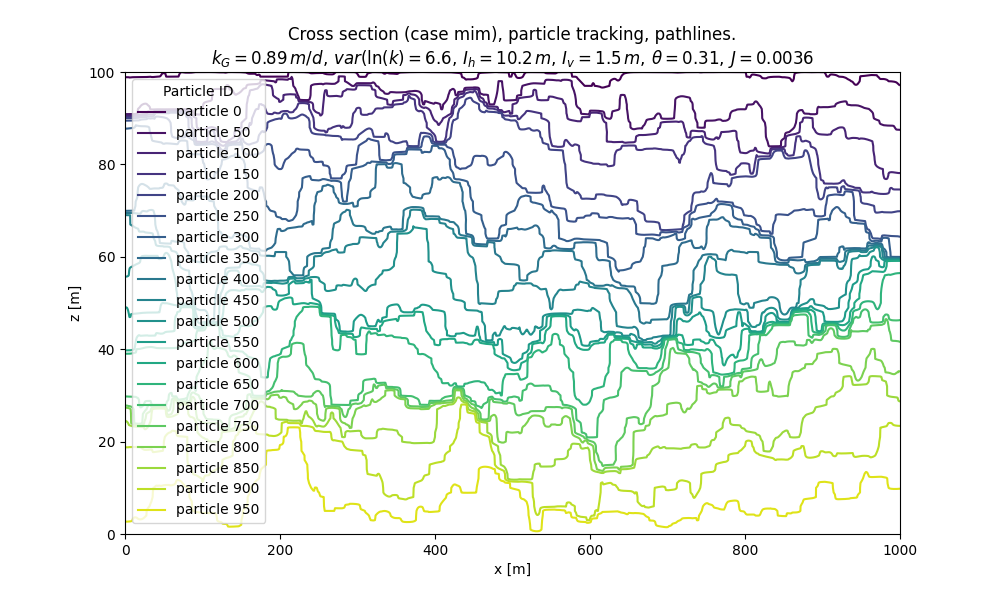
\includegraphics[width=0.8\textwidth]{/Users/Theo/GRWMODELS/python/mf6lab/Projects/Dispersion/cases/wimsaquif/images/plines_mim}

\caption{\label{fig:mim-paths}Modpath-computed pathlines.}

\end{figure}

\begin{figure}[H]
\centering
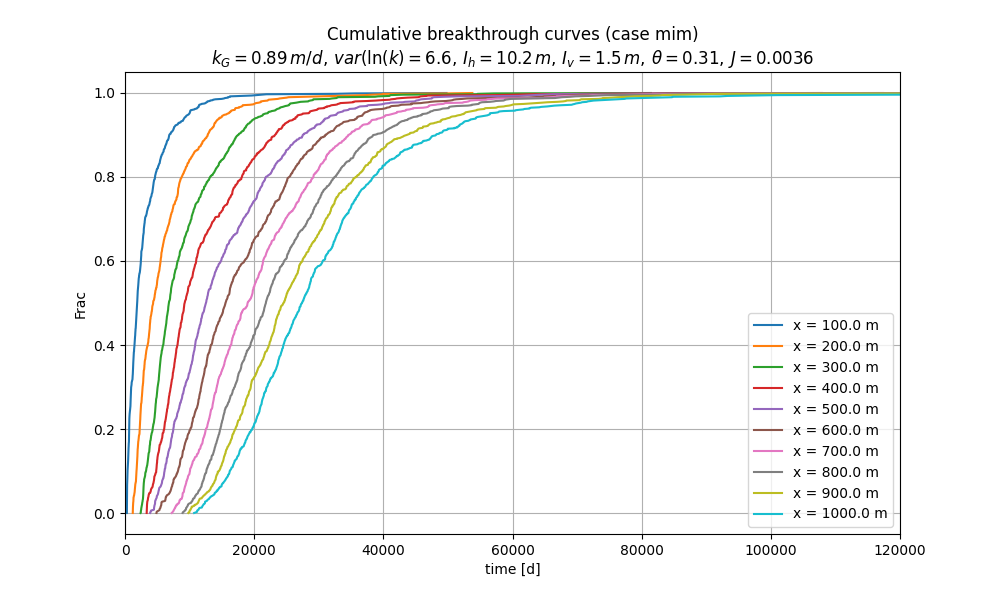
\includegraphics[width=0.8\textwidth]{/Users/Theo/GRWMODELS/python/mf6lab/Projects/Dispersion/cases/wimsaquif/images/cumul_t_mim}

\caption{\label{fig:mim-cum-t}Computed cumulative break-through curves}

\end{figure}

\begin{figure}[H]
\centering
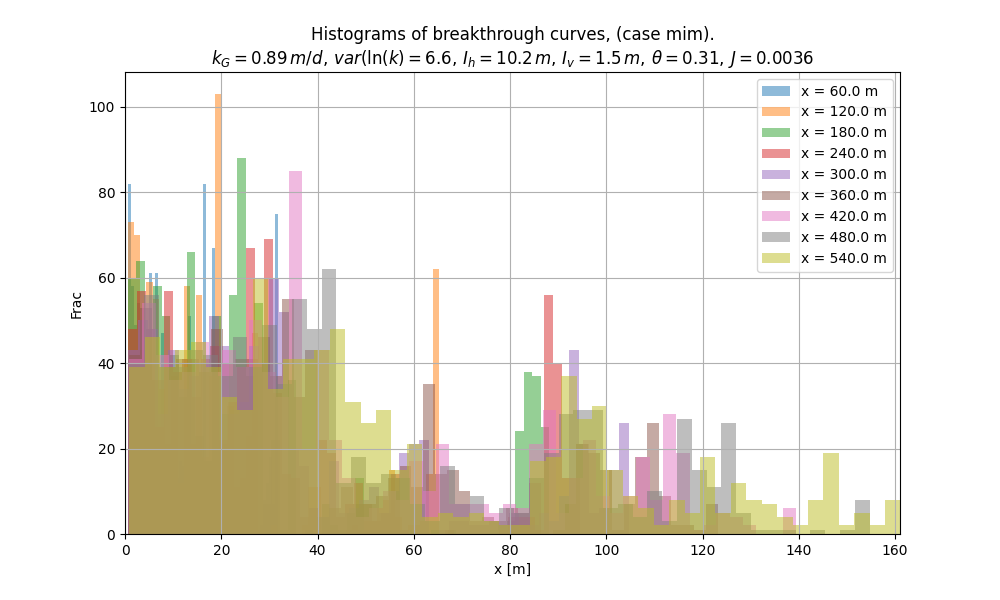
\includegraphics[width=0.8\textwidth]{/Users/Theo/GRWMODELS/python/mf6lab/Projects/Dispersion/cases/wimsaquif/images/hist_x_mim}

\caption{\label{fig:mim-hist_t}Computed break-through histograms}

\end{figure}

\begin{figure}[h]
\centering
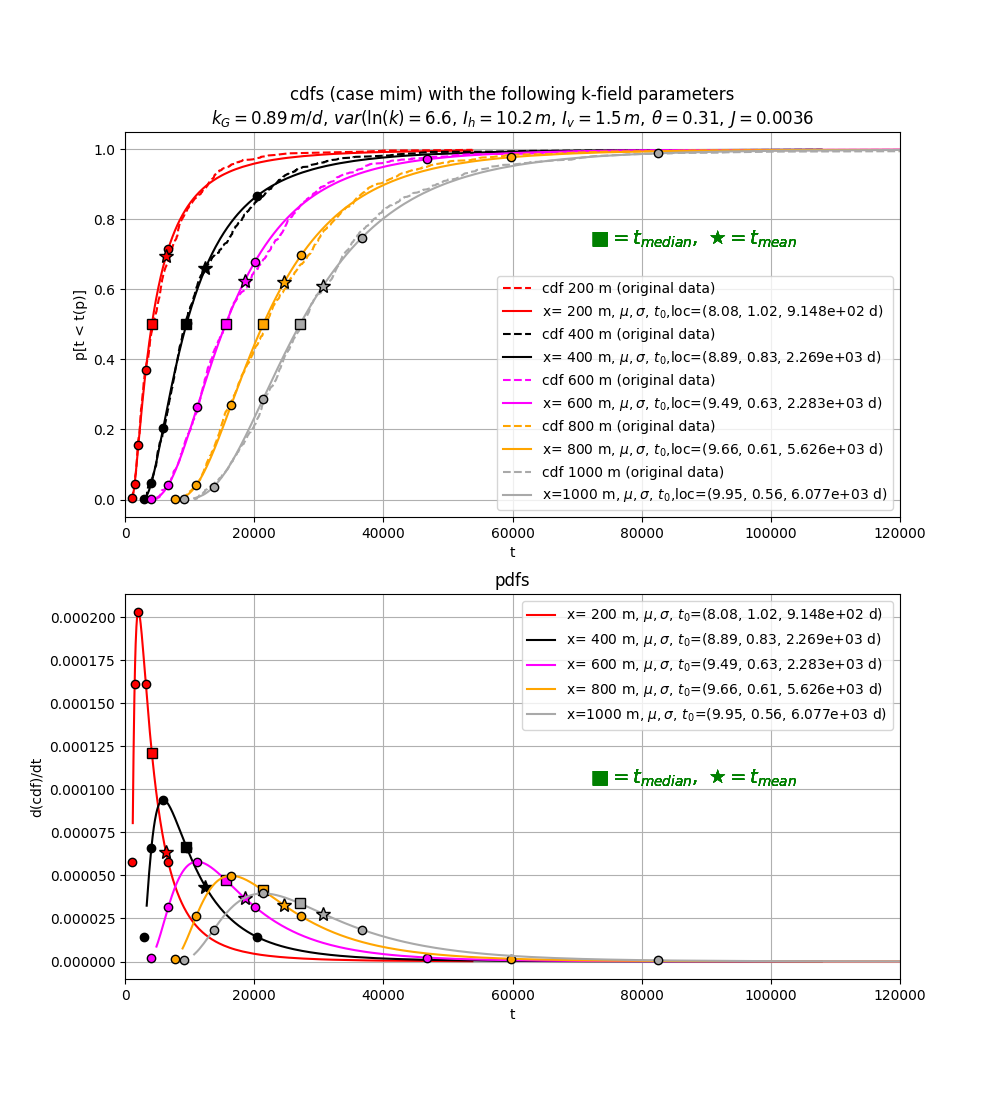
\includegraphics[width=0.8\textwidth]{/Users/Theo/GRWMODELS/python/mf6lab/Projects/Dispersion/cases/wimsaquif/images/BTanalysis_t_mim}

\caption{\label{fig:mim-BT_t}Top: Breakthrough curves with fitted cdf for
lognormal distrubiton. Bottom their pdf. The median and the mean are
given and the points at 0.2, 0.5, 1.0, 2 and 5 times $t_{mode}-t_{0}$
which provide a better insght with the lognormal distribution than
the usual quantiles of the cdf. Because of the skewness, $t_{mode}<t_{med}<t_{mean}$.
The skewed character of the breakthrough curves are clearly visible.
The maximum time is about 5 times the minimum time in this case. The
$t_{mode}$ at $xObs=200$ m is at about 400 d.}

\end{figure}

\begin{figure}[h]
\centering
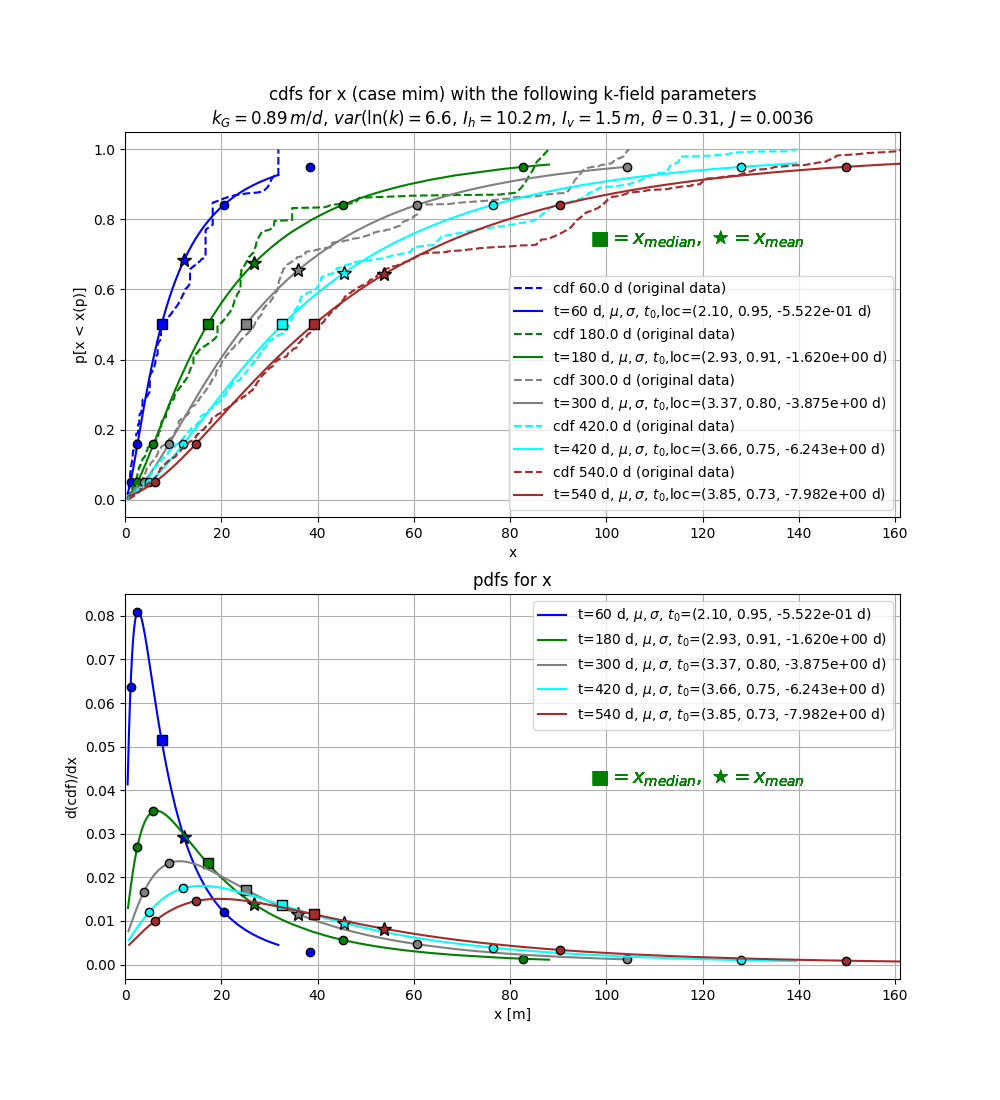
\includegraphics[width=0.8\textwidth]{/Users/Theo/GRWMODELS/python/mf6lab/Projects/Dispersion/cases/wimsaquif/images/BTanalysis_x_mim}

\caption{\label{fig:mim-BT-x}Top: Cumulative distribution of particles with
their fitted cdf at given observation times. Bottom their pdf. Shown
are $x_{median}$ and $x_{mean}$. Notice that $x_{mod}<x_{median}<x_{mean}$
for the lognormal distribution. Also show are the points for cdf =
0.05, 0.16, 0.5, 0.84 and 0.95. These work better than the mode-related
values above as the distribution for the $x$-values is less skewed
than for the $t$-values.}

\end{figure}


\subsection{The same cross section with the same parameters except for a much
lower variance of the conductivity, namely $var(\ln\left(k\right))$
is 1.1 instead of 6.6}

The more homogeneous the aquifer, the more the breakthrough will conform
to Fickian or Gaussian character with more symmetrical breakthrough
curves and histograms. We can test this with the same model by just
changing the variance of the $\ln\left(k\right)$ field from 6.6 in
the previous case to $1.5$, a value which I deem more realistic for
the more homogeneous aquifers found in the Netherlands. The results
are given in the figures below. Figure \ref{fig:mim11-kfield} looks
similar to figure \ref{fig:mim-kfield}, however, the colorbar below
it shows that the values are different, and less extreme. Figure \ref{fig:mim11-stream}
shows that although the streamlines still go up and down along their
paths, these fluctuations are now much less than those in figure \ref{fig:stream-function}.
Also, the head contours are much more straight in figure \ref{fig:mim11-stream}
than in figure \ref{fig:stream-function}. This is also due to the
more homogeneous aquifer that we created in this section. As expected,
the cumulative breakthrough curves now show much more symmetry about
the 50\% value, with far a less extreme tail. In fact, except for
the small asymmetry in the last curve for $x=1000$ m, asymmetry are
essentially absent for all shorter travel distances. Hence, all breakthrough
curves are now essentially Gaussian. The symmetry of the breakthough
behavior is also reveiled by the histograms and jumps into the eye
when comparing figure \ref{fig:mim11-t-hist} with figure \ref{fig:mim-hist_t}.

\begin{figure}[H]
\centering
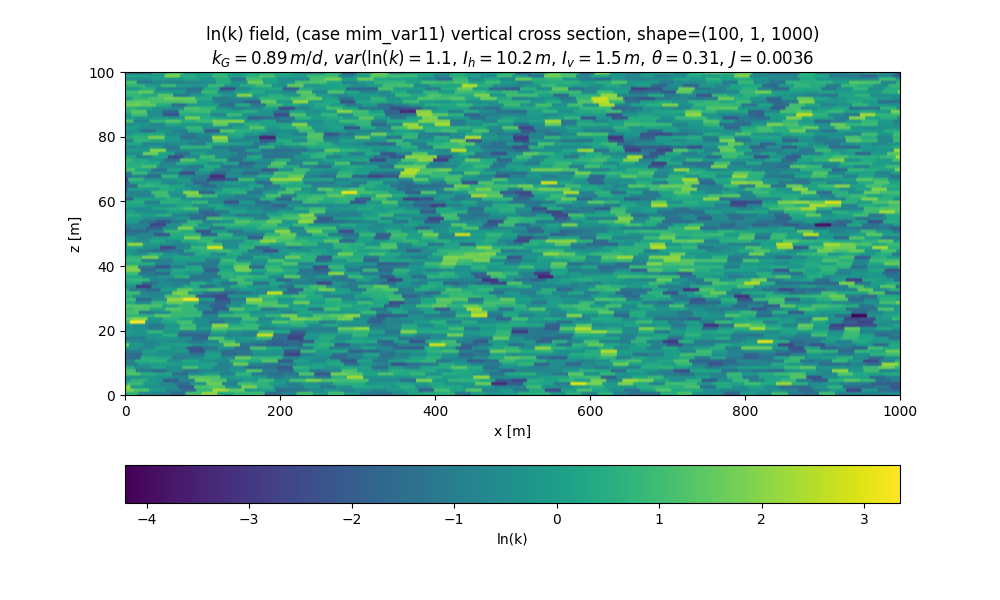
\includegraphics[width=0.8\textwidth]{/Users/Theo/GRWMODELS/python/mf6lab/Projects/Dispersion/cases/wimsaquif/images/kfield_mim_var11}

\caption{\label{fig:mim11-kfield}Image of the generated $ln\left(k\right)$
field for the cross section. For the rest the parameters are the same
as in the previous section}

\end{figure}

\begin{figure}[H]
\centering
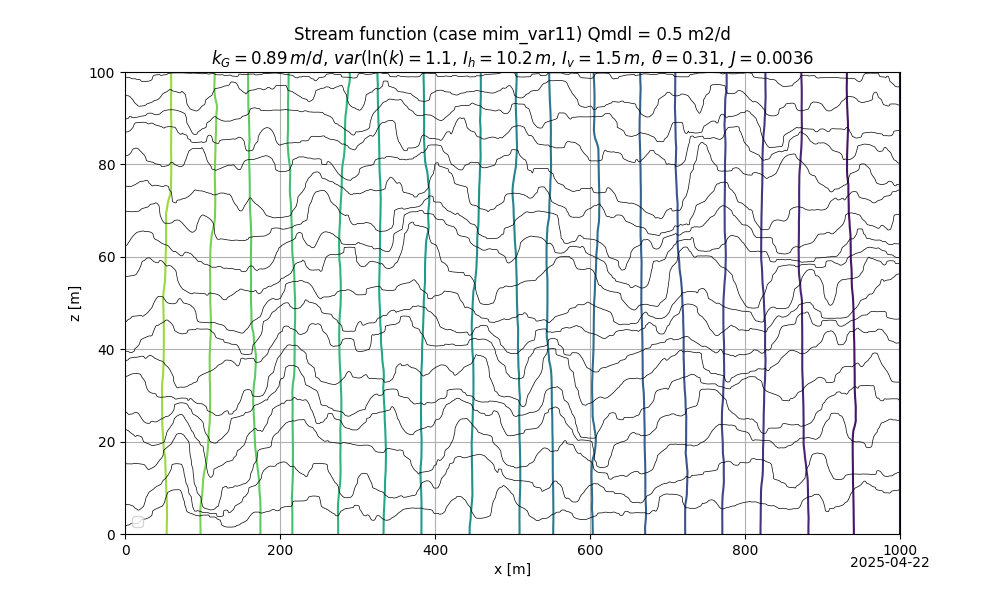
\includegraphics[width=0.8\textwidth]{/Users/Theo/GRWMODELS/python/mf6lab/Projects/Dispersion/cases/wimsaquif/images/stream_func_mim_var11}

\caption{\label{fig:mim11-stream}Srteamlines and head contours of the cross
section computed using Modflow.}

\end{figure}

\begin{figure}[H]
\centering
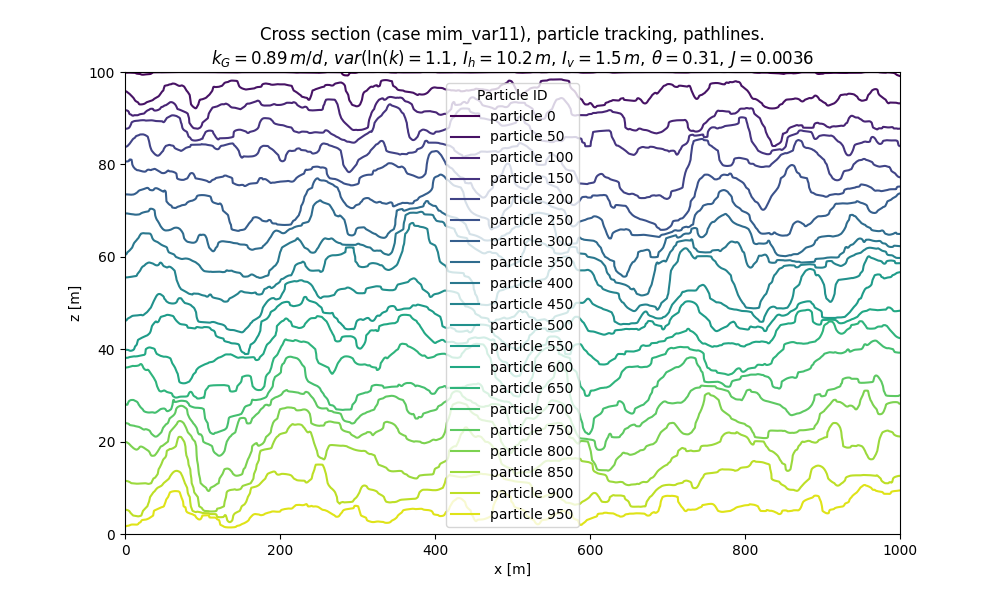
\includegraphics[width=0.8\textwidth]{/Users/Theo/GRWMODELS/python/mf6lab/Projects/Dispersion/cases/wimsaquif/images/plines_mim_var11}

\caption{\label{fig:mim11-paths}Pathlines, only every 5th particle is shown}

\end{figure}

\begin{figure}[H]
\centering
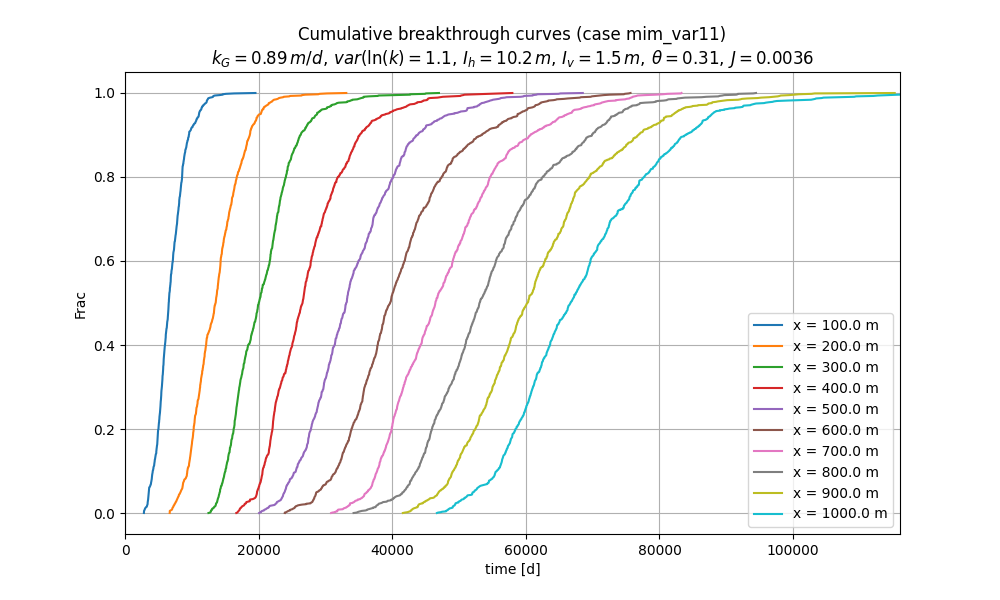
\includegraphics[width=0.8\textwidth]{/Users/Theo/GRWMODELS/python/mf6lab/Projects/Dispersion/cases/wimsaquif/images/cumul_t_mim_var11}

\caption{\label{fig:mimv11-t-cum}Cumulative break-through curves for different
locations in the cross section}

\end{figure}

\begin{figure}[H]
\centering
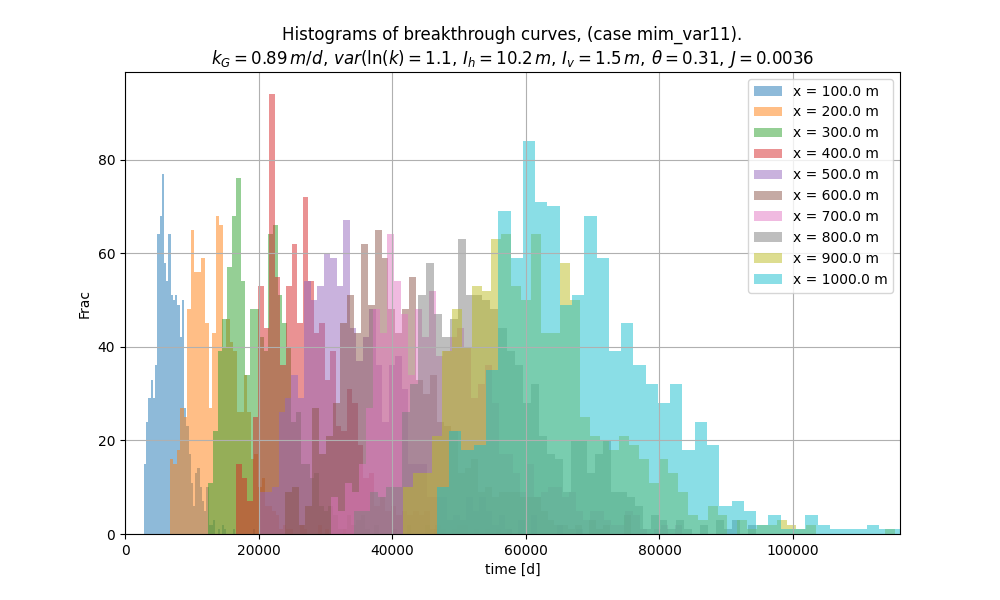
\includegraphics[width=0.8\textwidth]{/Users/Theo/GRWMODELS/python/mf6lab/Projects/Dispersion/cases/wimsaquif/images/hist_t_mim_var11}

\caption{\label{fig:mim11-t-hist}Histogams for the break-through at different
locations long the cross section as computed from the cumulatives.}

\end{figure}

\begin{figure}[h]
\centering
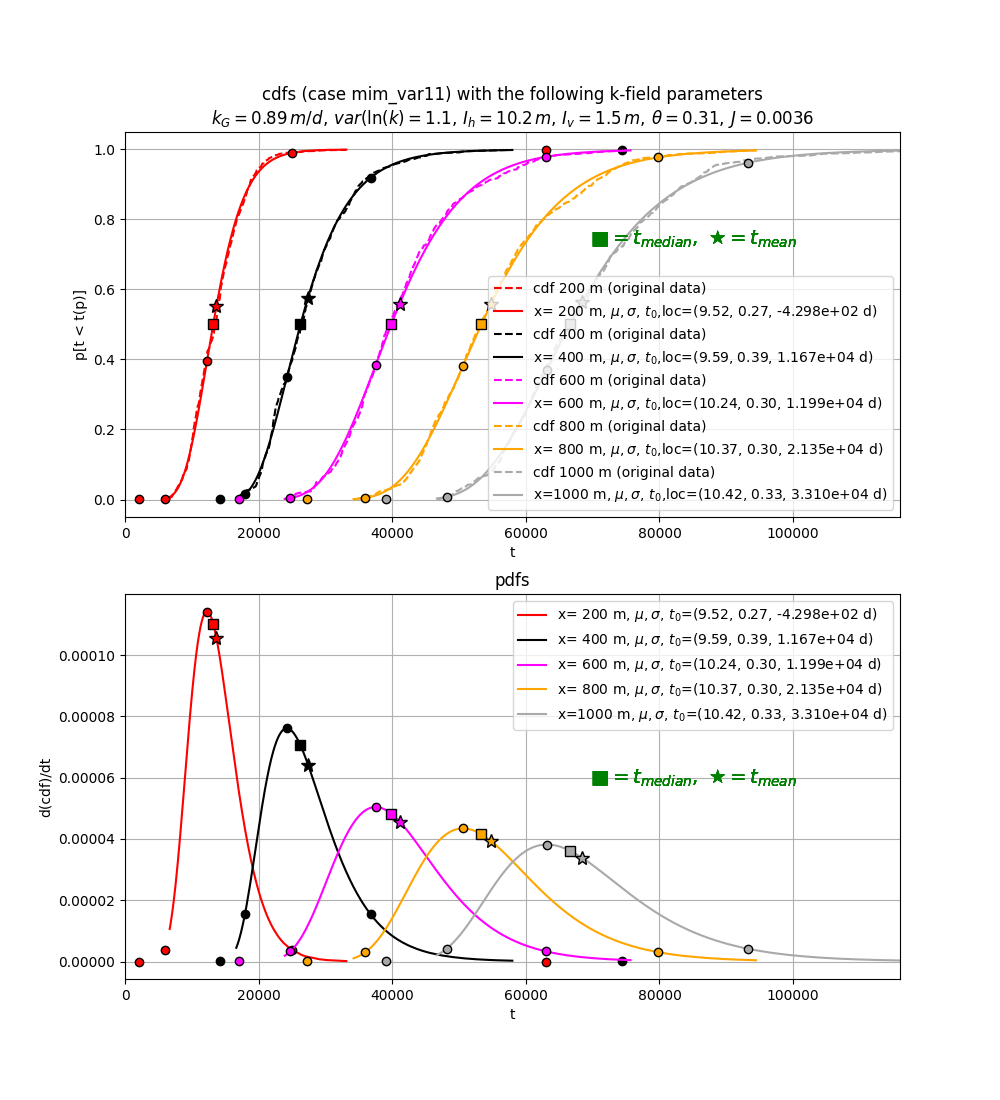
\includegraphics[width=0.8\textwidth]{/Users/Theo/GRWMODELS/python/mf6lab/Projects/Dispersion/cases/wimsaquif/images/BTanalysis_t_mim_var11}

\caption{\label{fig:mim11-BT-t}Top: Breakthrough times and fitted log-normal
cdfs for same case as before by $var\left(\ln\left(k\right)\right)=1.2$
instead of $6.6$. Bottom: pdf's. Note the dots are at 0.2, 0.5, 1.0,
2.0 and 5.0 times $t_{mode}$. These are here less insightful because
the distrubtions are far less skewed than in the previous case with
the much larger $var\left(\ln\left(k\right)\right)$ value of 6.6
instead of 1.1. The maximum time is about 3 times the minimum time
in this case. $t_{mode}$ at $xObs=200$ m is about 15000 days, which
is about 4 times later than in the previous case. Also the mean time
is larger now. At $x_{Obs}=1000$ m it is now about 75000 days while
in the previous case it was about 38000 days, shorter due to higher
conductivities in the longest heterogeneities.}

\end{figure}

\begin{figure}[h]
\centering
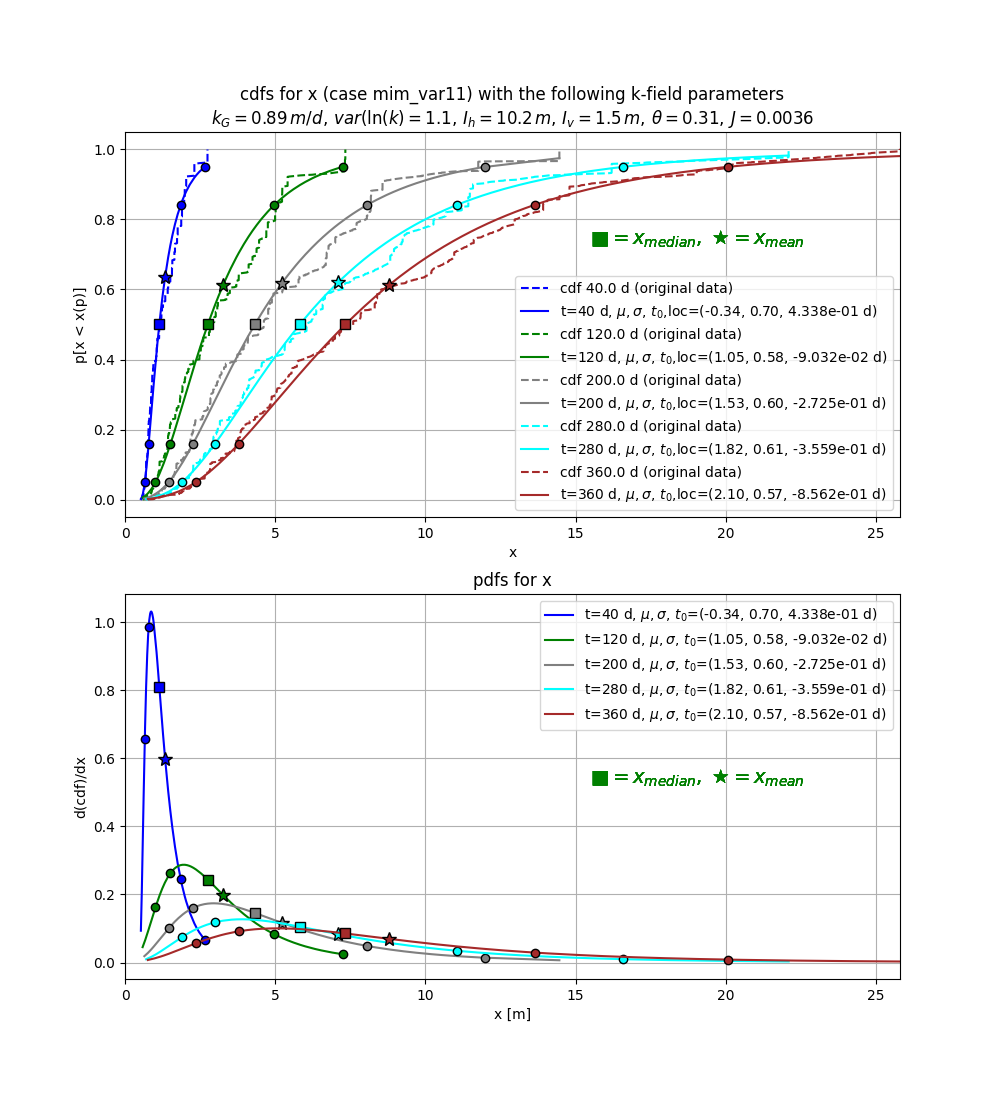
\includegraphics[width=0.8\textwidth]{/Users/Theo/GRWMODELS/python/mf6lab/Projects/Dispersion/cases/wimsaquif/images/BTanalysis_x_mim_var11}

\caption{\label{fig:mim11-BT-x}Distribution curves for the particles and fitted
lognormal distribution for cdf and pdf.}

\end{figure}


\subsection{Regular conductivity field as exponential random field with the same
parameters as used in the MIM model of section \ref{subsec:Made-cross-section}.}

The MIM model to simulate the MADE breakthrough curves in \cite{Fiori13}
uses blocks of width $2R$, essentially $2I_{h}$ with each having
a constant conductivity throughout the block, while these block conductivities
area conform the statistics for $\ln\left(k\right)$, for $var\left(\ln\left(k\right)\right)$
and for the integration lengths $I_{h}$ and $I_{v}$. Instead of
using blocks, it may be feasible to simply generate a cross-section
that fulfills these condictions but without resorting to the blocks
of the MIM model. The cross section generated this way, is shown in
figure \ref{fig:gaus-kfield}. It lacks the block structure, which
characterizes the cross section of figure \ref{fig:mim-kfield}. The
stream and head lines in figure \ref{fig:gaus-stream} are as irregular
as in figure \ref{fig:stream-function}, which is due to the same
large log-conductivity variance used in these two cases. Figure \ref{fig:gaus-cum-t}
shows the breakthrough curves. The top figure shown those belonging
to the current conductivity field, while, for easy comparison, the
bottom figure is the same as figure \ref{fig:mim-cum-t} for the model
with the block structure, but otherwise the same parameters. Figure
\ref{fig:gaus-cum-t} makes clear that, also with a fully continuous
random field with exponential covariance, similar breakthrough curves
are obtained as with a MIM-type model with blocks. Probably it is
just the applied range of the horizontal and vertical variograms that
matter to get a behavior characteristic of preferential flow path,
while it does matter little if a block structure is added. Figure
\ref{fig:gaus-hist-t}, on top, shows the histograms derived from
the breakthrough curves for this continuous cross section, and at
the bottom, again for easy comparison, those obtained with the block
structure and otherwise the same parameters already shown in figure
\ref{fig:mim-hist_t}. I would argue that both figures are not too
different. They are essentially characterized by asymmetry with a
large tail, which is what one expects from a strongly heterogeneous
aquifer.

\begin{figure}[H]
\centering
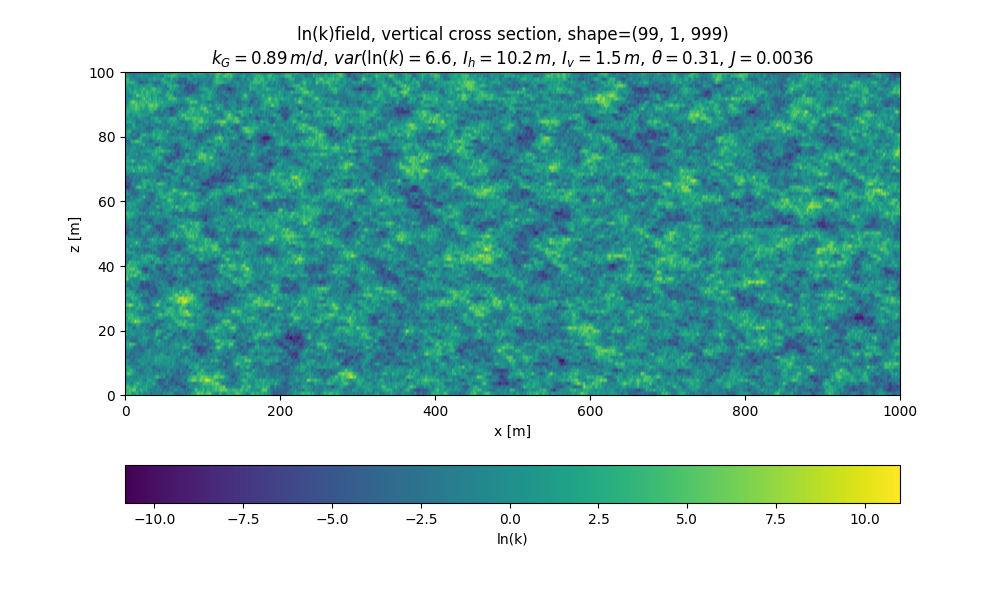
\includegraphics[width=0.8\textwidth]{/Users/Theo/GRWMODELS/python/mf6lab/Projects/Dispersion/cases/wimsaquif/images/kfield_gaus}

\caption{\label{fig:gaus-kfield}Generated ln(k) field using exponential model
with variance and $x_{len}=I_{h}$ and $z_{len}=I_{v}$, and the parameters
given in the header of the figure.}

\end{figure}

\begin{figure}[H]
\centering
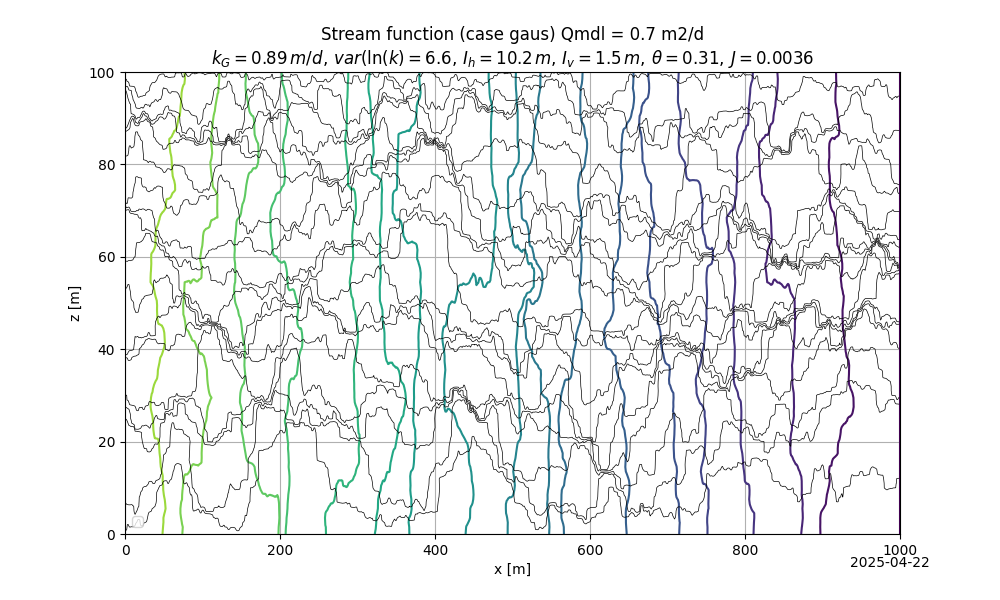
\includegraphics[width=0.8\textwidth]{/Users/Theo/GRWMODELS/python/mf6lab/Projects/Dispersion/cases/wimsaquif/images/stream_func_gaus}

\caption{\label{fig:gaus-stream}Stream function and head contours after simulating
the cross section with the conductivity field in the previous figure.}

\end{figure}

\begin{figure}[H]
\centering
Exponential random field field

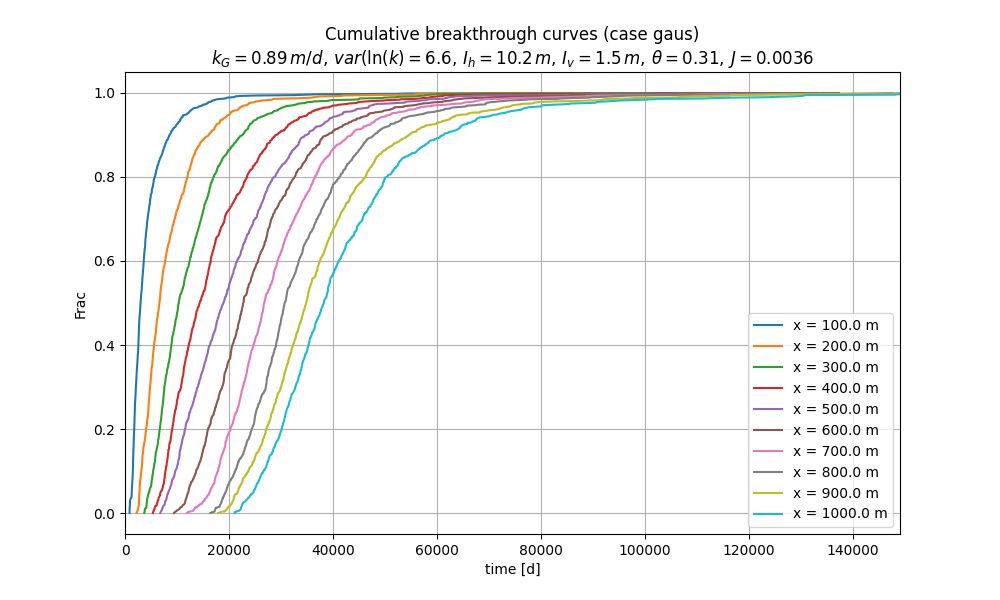
\includegraphics[width=0.8\textwidth]{/Users/Theo/GRWMODELS/python/mf6lab/Projects/Dispersion/cases/wimsaquif/images/cumul_t_gaus}

MIM blocks field (using the same expnential field parameters)

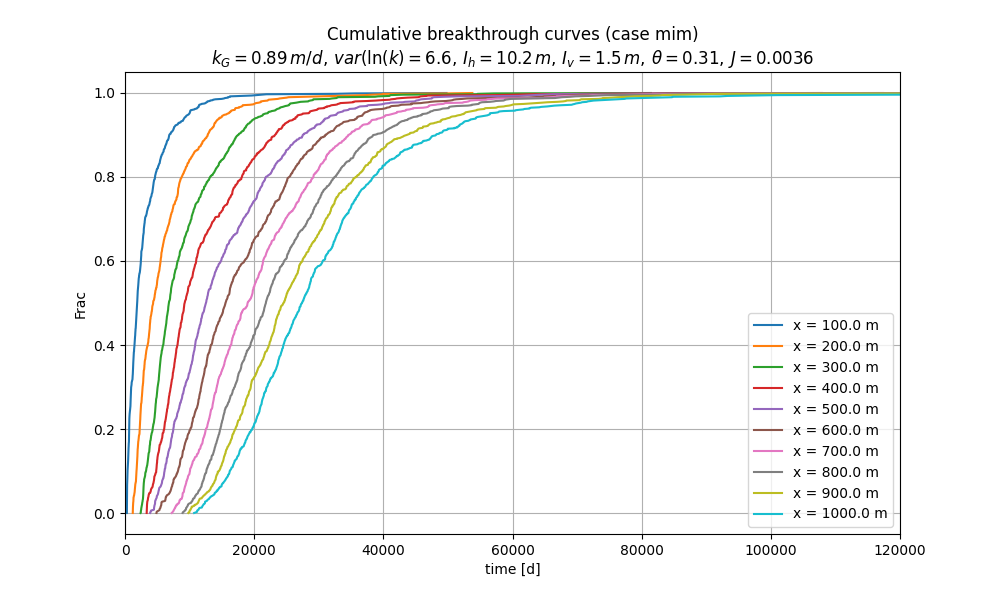
\includegraphics[width=0.8\textwidth]{/Users/Theo/GRWMODELS/python/mf6lab/Projects/Dispersion/cases/wimsaquif/images/cumul_t_mim}

\caption{\label{fig:gaus-cum-t}Breakthorugh curves compute using Modpath.}

\end{figure}

\begin{figure}[H]
\centering
Exponential random field

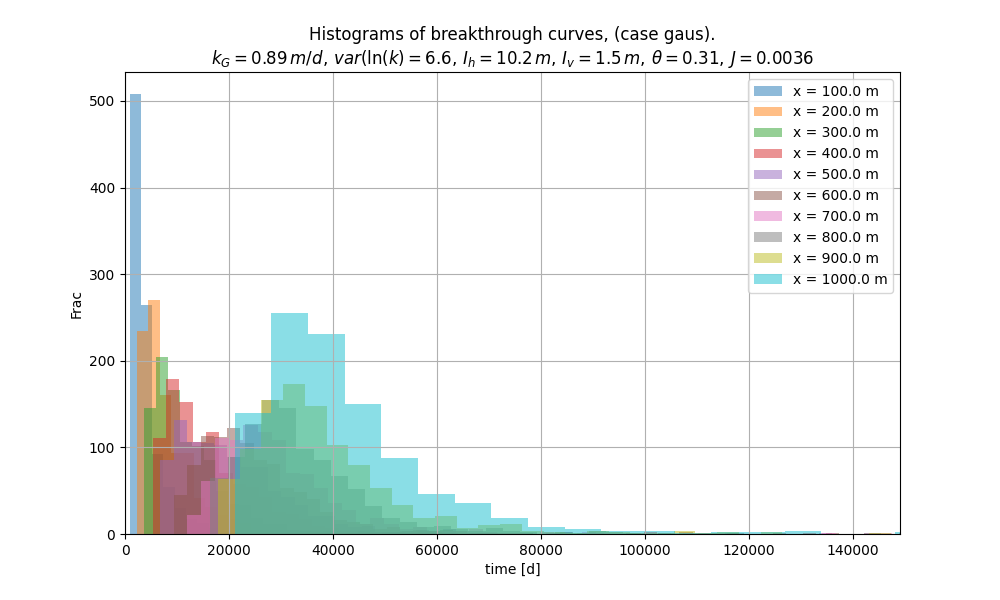
\includegraphics[width=0.8\textwidth]{/Users/Theo/GRWMODELS/python/mf6lab/Projects/Dispersion/cases/wimsaquif/images/hist_t_gaus}

MIM block field with the same exponential random field parameters

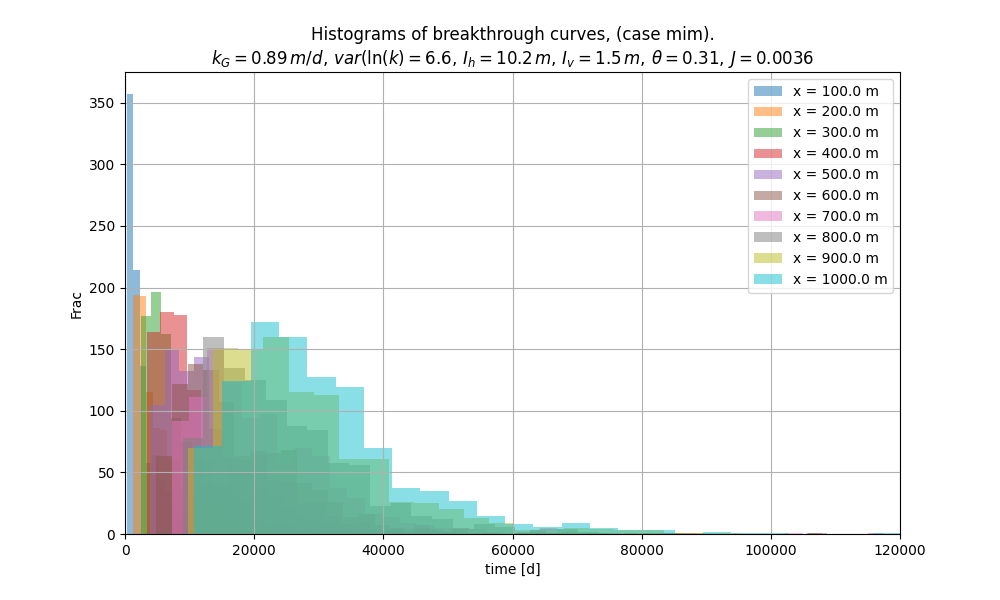
\includegraphics[width=0.8\textwidth]{/Users/Theo/GRWMODELS/python/mf6lab/Projects/Dispersion/cases/wimsaquif/images/hist_t_mim}

\caption{\label{fig:gaus-hist-t}Histograms derived from the breakthrough curves
in figure \ref{fig:gaus-cum-t}}

\end{figure}

\begin{figure}[h]
\centering
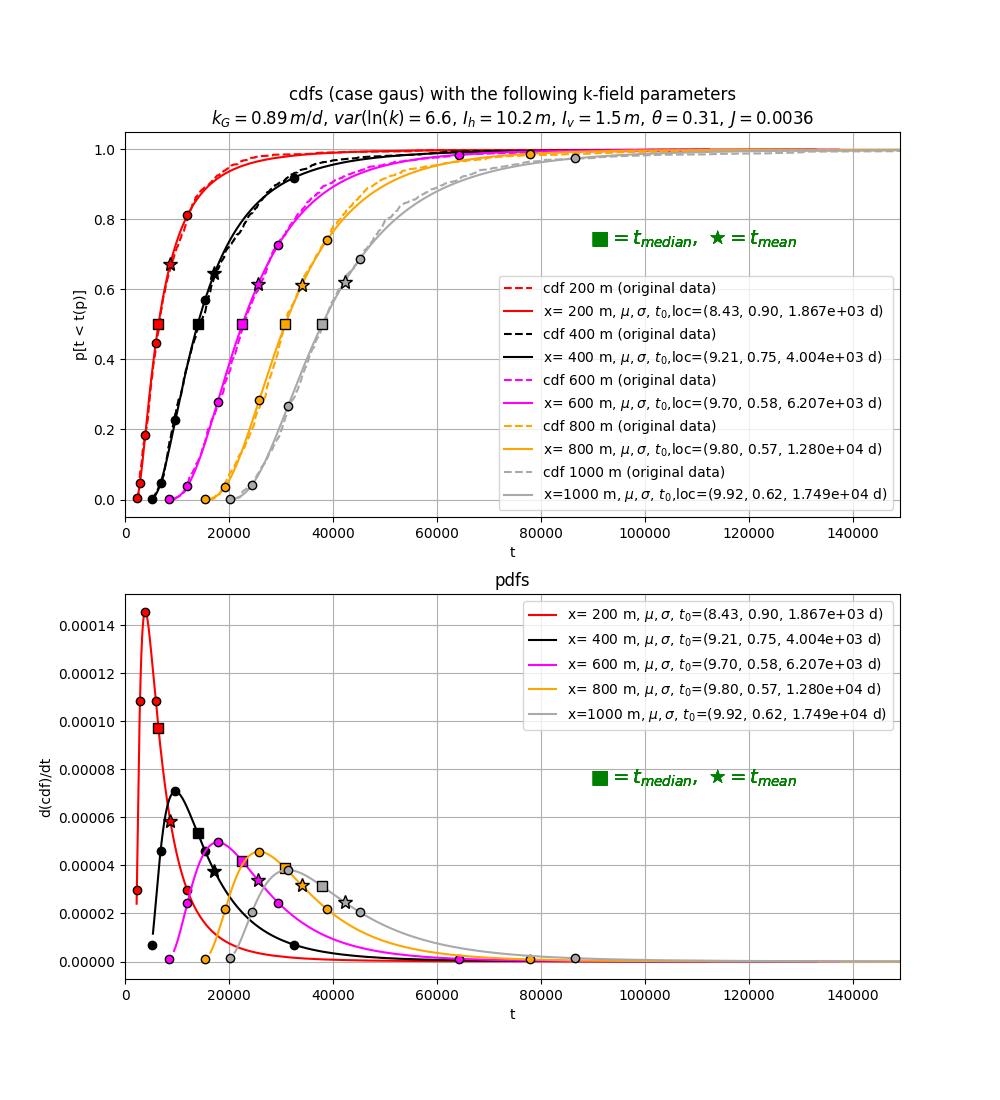
\includegraphics[width=0.8\textwidth]{/Users/Theo/GRWMODELS/python/mf6lab/Projects/Dispersion/cases/wimsaquif/images/BTanalysis_t_gaus}

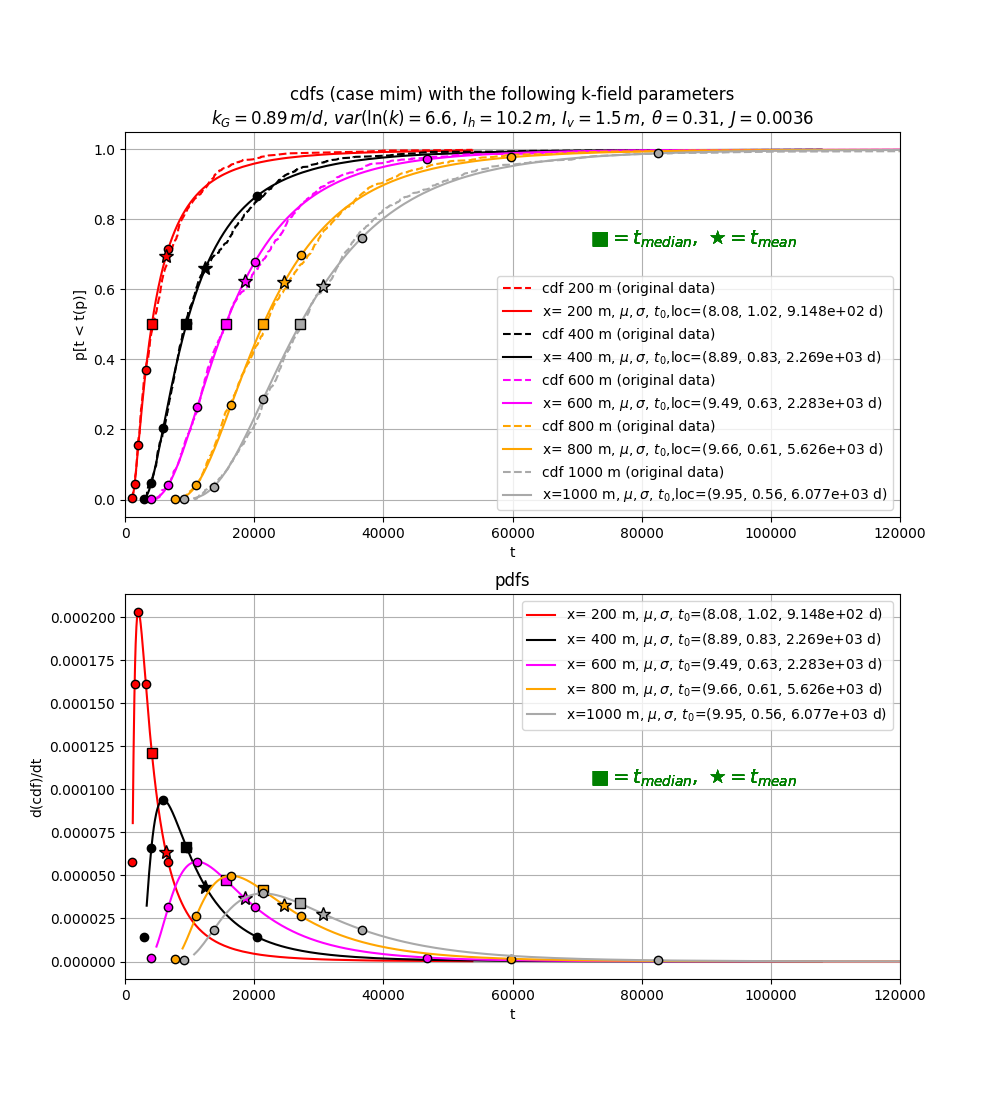
\includegraphics[width=0.8\textwidth]{/Users/Theo/GRWMODELS/python/mf6lab/Projects/Dispersion/cases/wimsaquif/images/BTanalysis_t_mim}

\caption{\label{fig:gaus-BT-t}}

\end{figure}

\begin{figure}[h]
\centering
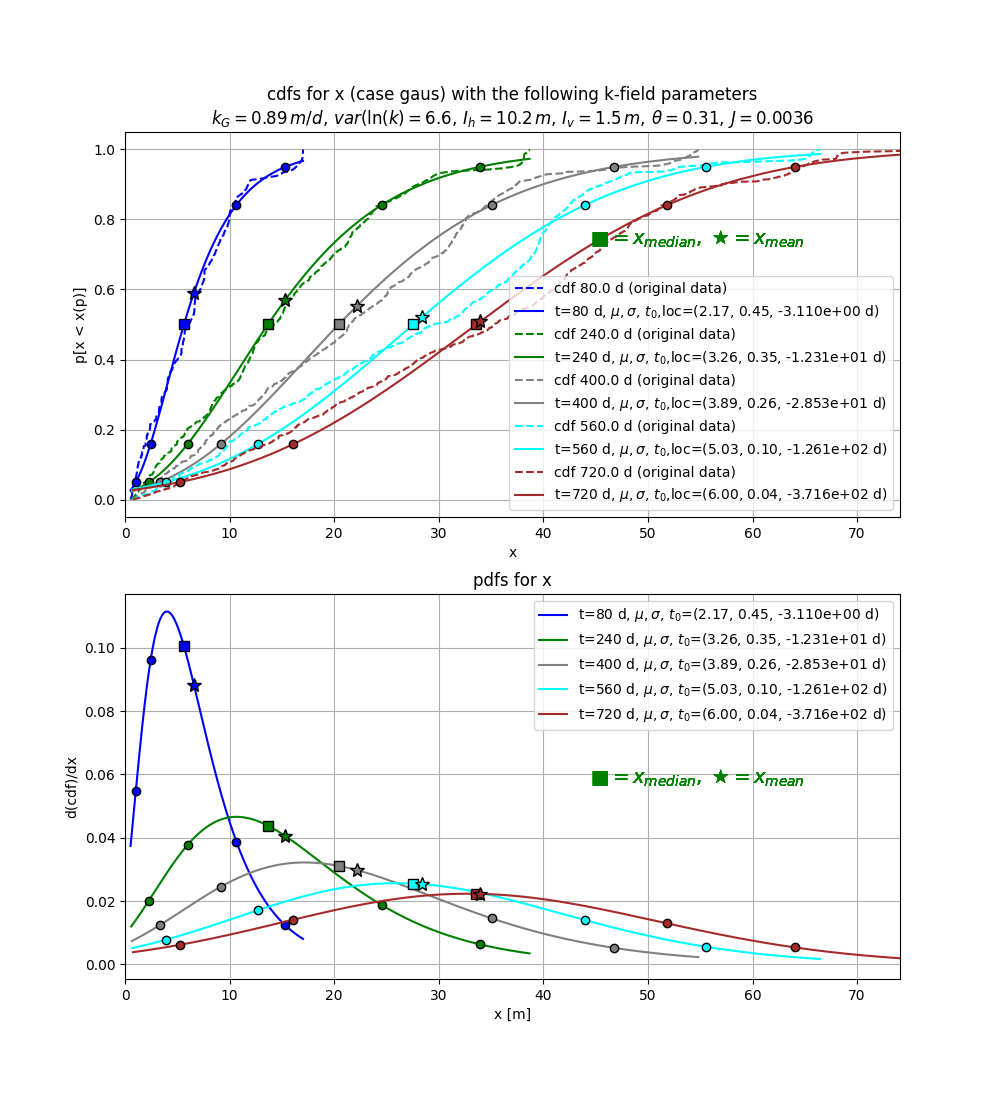
\includegraphics[width=0.8\textwidth]{/Users/Theo/GRWMODELS/python/mf6lab/Projects/Dispersion/cases/wimsaquif/images/BTanalysis_x_gaus}

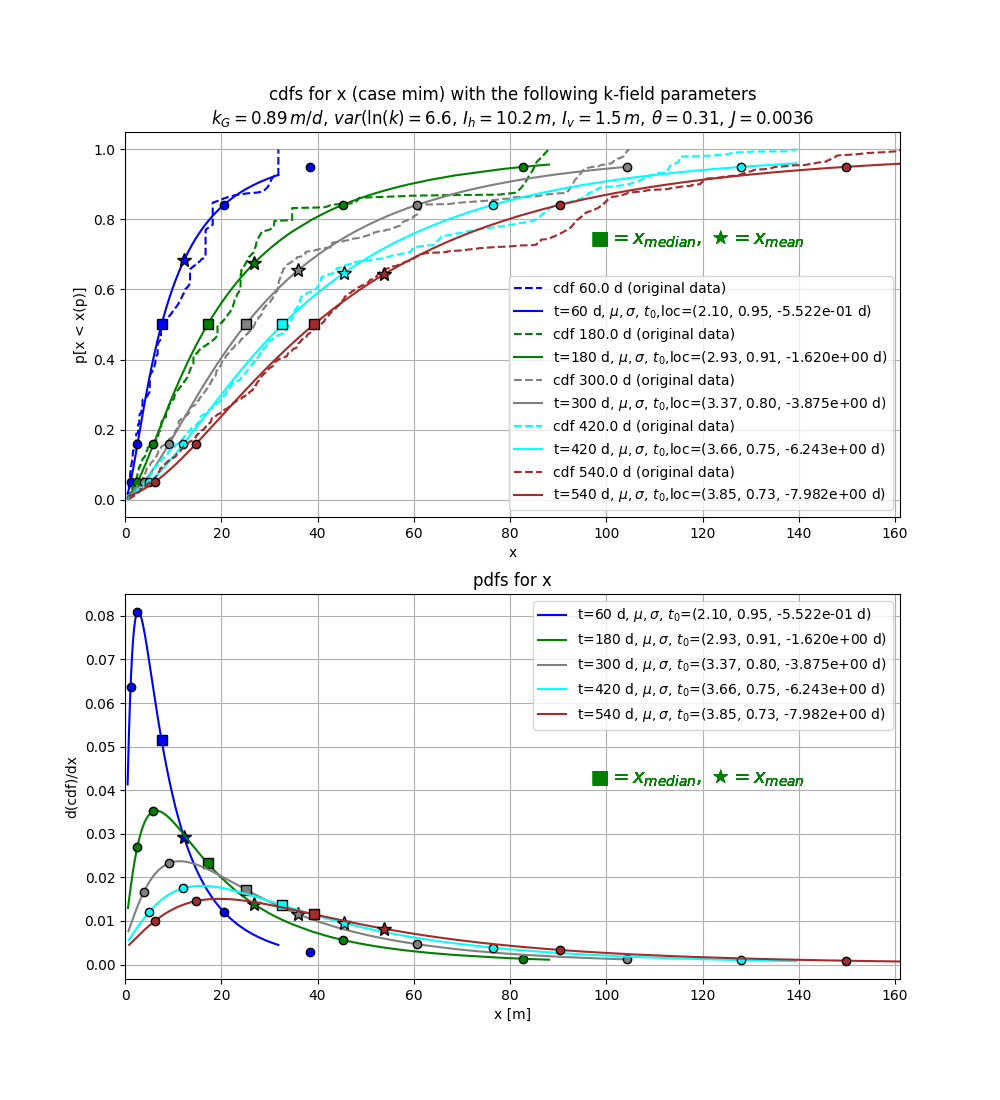
\includegraphics[width=0.8\textwidth]{/Users/Theo/GRWMODELS/python/mf6lab/Projects/Dispersion/cases/wimsaquif/images/BTanalysis_x_mim}

\caption{\label{fig:gaus-BT-x}}

\end{figure}


\section{Wim's aquifer}

In his papers, \nocite{Lange20,Lange22,Lange25} simulates the dispersion
using an artificial aquifer built of blocks, he calls domains of given
size that are place next to each other and on top of each other as
to fill the entire cross section of the aquifer. Each block as a low
background conductivity and includes an elongated facies with a high
conductivity. The background and high facies conductivities are the
same in each block. For this example they are chose to be 5 and 500
m/d respectively.

Like in the previous examples the cross section has the same size,
100 m deep and 1000 m wide with cells of 1x1 m$^{2}$. Each block
was given the size of 20 cells along the x-axis and 5 cells along
the z-axis. The facies was placed randomly inside each block. The
inner facies was given the size of 20 cells along the x-axis and 1
cell along the z-axis. This is about what De Lange uses in his example
pictures. The boundary conditions are the same as in the previous
examples, a gradient of 0.0036 and a porosity of 0.31. The results
of the simulation are in the following pictures. Figure \ref{fig:wdl-kfield}
shows the $\ln\left(k\right)$ field, i.e. one background conductivity
and one facies conductivity according to the header of the figure.
Figure \ref{fig:wdl-stream} shows the streamline and the head contours.
The high-conductive inclusions clearly distort and channel the flow
through them. Figure \ref{fig:wdl-cum-t} shows the cumulative breakthrough
curves for different locations along the cross section. They are not
symmetric due to the hetergeneous character of the aquifer. However,
the asymmetry of the time-breakthrough curves at different observation
locations can be deemed not so high as expected. The same conclusion
can be drawn from the histograms in figure \ref{fig:wdl-hist-t} they
are far less asymmetric than expected. Therefore, they might be reasonably
modelled by a more traditional Fickian model. Perhaps the number of
inclusions or their lengths are to small to deem this aquifer a really
heterogeneous despite the large contrast between the background and
the facies conductivities.

The breakthrough curves for the different observation distances in
the top of figure \ref{fig:gaus-BT-t} show that the lognormal distribution
fits very well through the modeled breakthrough curves. The corresponding
pdfs at the bottom of figure \ref{fig:gaus-BT-t} also show only moderate
skewness. Perhaps strangely enough, the breakthrough curves (or cumulative
location curves) for different observation times in the top of figure
\ref{fig:gaus-BT-x} don't fit well to the lognormal distribution.
There shape reveils the effect of preferential flow paths in these
graphs that show the location of the particles at different moments.
The corresponding pdfs are strongly skewed, contrary to those in figure
\ref{fig:gaus-BT-t}. The skewness of the pdfs enveils the preferential
flow paths with a limited part of the flow traveling at a high rate
and the bulk lagging behind at a low rate caused by the 100 times
lower background conductivities applied in this example. Yet figure
\ref{fig:gaus-BT-x} also shows that the distances traveled at the
different observation times are small compared to the length of the
cross section of 1000 m. This contrasts largely from the distance
travelled by the particles capatured at the different observation
locations which varied from 100, 200, ... 1000 m and was the same
for all particles at each given distance. This may imply the for the
small distances the mixing as a process is too limited, given the
length of the inclusions of 20 m. The very strong skewed character
of the pdfs for the different observation times, which represent the
most likely distribution of the pollution plume released at $t=0$
and $x=0$ bare a large comparison to the large skewness in obsevered
plume spreading in heterogeneous locations as the Made site. 

On thing to do is to set up the cross section in this example according
to the theory of \cite{Lange20,Lange22,Lange25} such that it reflects
the properties at the Made site.

\begin{figure}[H]
\centering
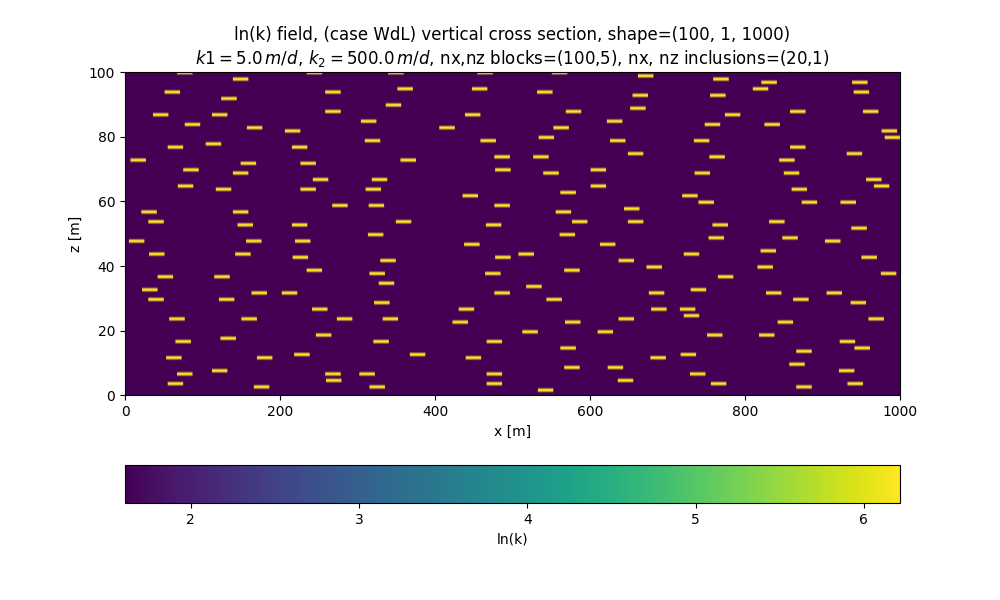
\includegraphics[width=0.8\textwidth]{/Users/Theo/GRWMODELS/python/mf6lab/Projects/Dispersion/cases/wimsaquif/images/kfield_WdL}

\caption{\label{fig:wdl-kfield}Conductivity field with background and facies
data given in the header.}

\end{figure}

\begin{figure}[H]
\centering
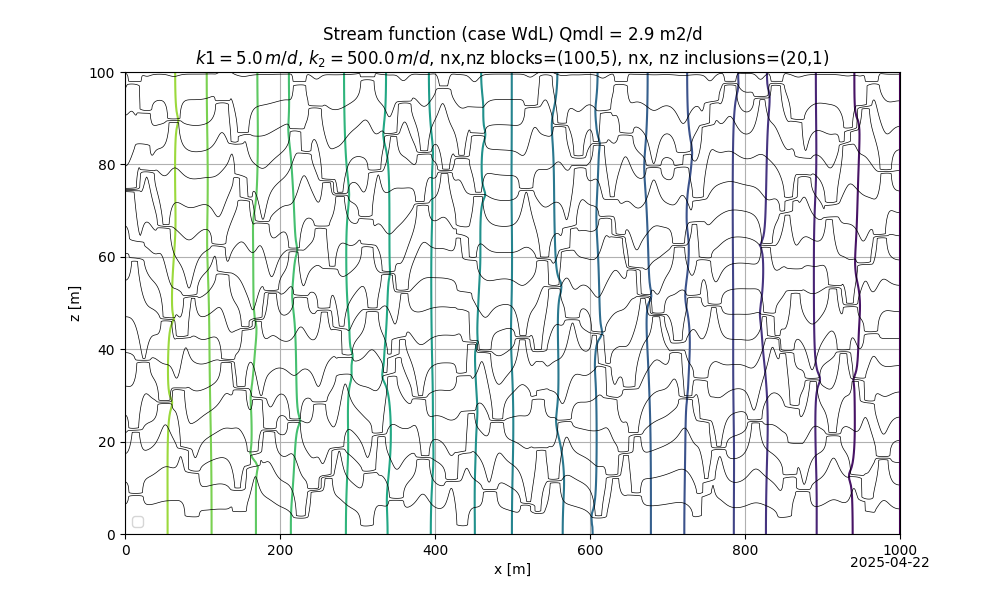
\includegraphics[width=0.8\textwidth]{/Users/Theo/GRWMODELS/python/mf6lab/Projects/Dispersion/cases/wimsaquif/images/stream_func_WdL}

\caption{\label{fig:wdl-stream}Streamlines and head contours for the simulated
cross section. Only every 5th particle is shown.}
\end{figure}

\begin{figure}[H]
\centering
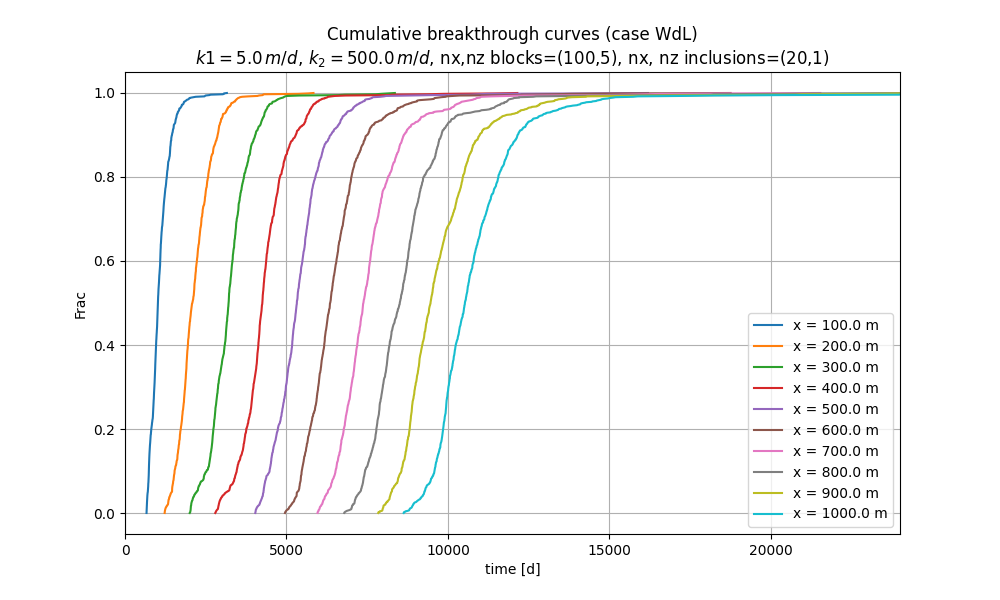
\includegraphics[width=0.8\textwidth]{/Users/Theo/GRWMODELS/python/mf6lab/Projects/Dispersion/cases/wimsaquif/images/cumul_t_WdL}

\caption{a\label{fig:wdl-cum-t}Cumulative breakthrough curves at different
locations along the cross section}

\end{figure}

\begin{figure}[H]
\centering
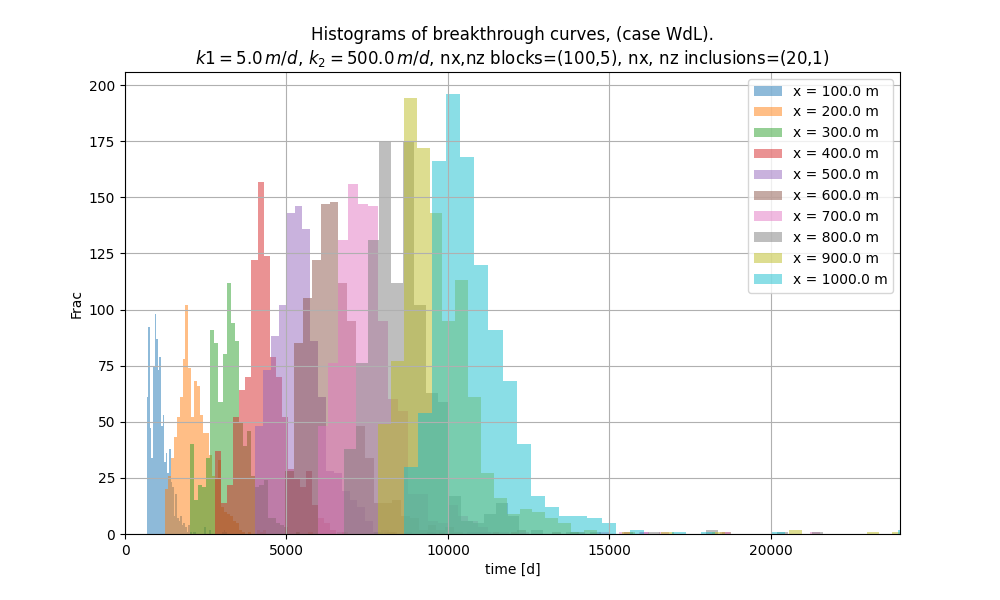
\includegraphics[width=0.8\textwidth]{/Users/Theo/GRWMODELS/python/mf6lab/Projects/Dispersion/cases/wimsaquif/images/hist_t_WdL}

\caption{\label{fig:wdl-hist-t}Histograms of different breakthrough points
along the cross section}

\end{figure}

\begin{figure}[h]
\centering
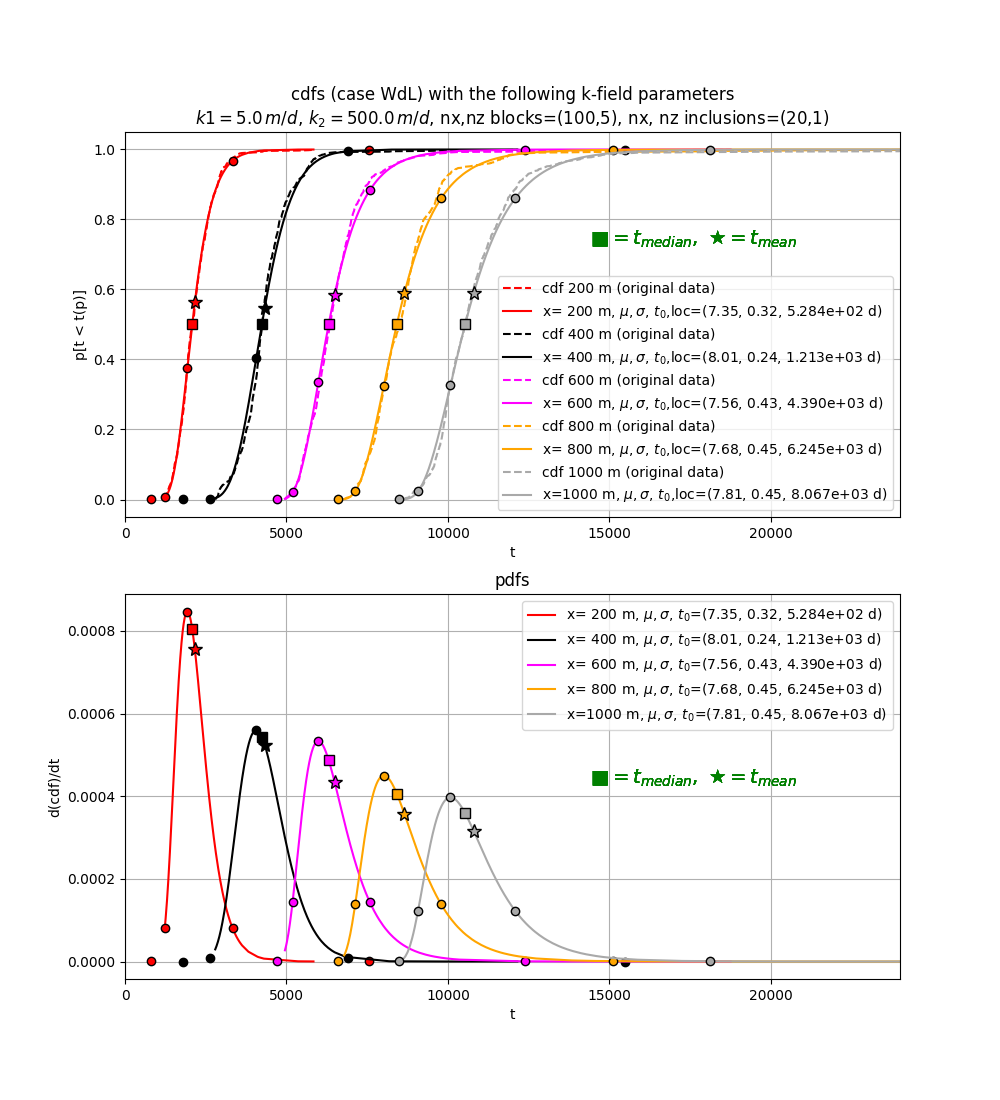
\includegraphics[width=0.8\textwidth]{/Users/Theo/GRWMODELS/python/mf6lab/Projects/Dispersion/cases/wimsaquif/images/BTanalysis_t_WdL}

\caption{\label{fig:wdl-BT-t}Top: Breakthrough curves from the model and fitted
cdf's. Bottom: Pdfs corresponding to the fitted cdfs. Not that for
the lognormal distirbution $t_{mode}<t_{median}<t_{mean}$ as indicated.
The circles are plotted at 0.2, 0.5, 1.0, 2.0 and 5.0 times $t_{mode}-t_{0}$
where $t_{0}$ is the lowest possible value for the lognormal distribution
($t_{0}=loc)$ where $loc$ is one of the parameters given by the
fitting of the computed data.}

\end{figure}

\begin{figure}[h]
\centering
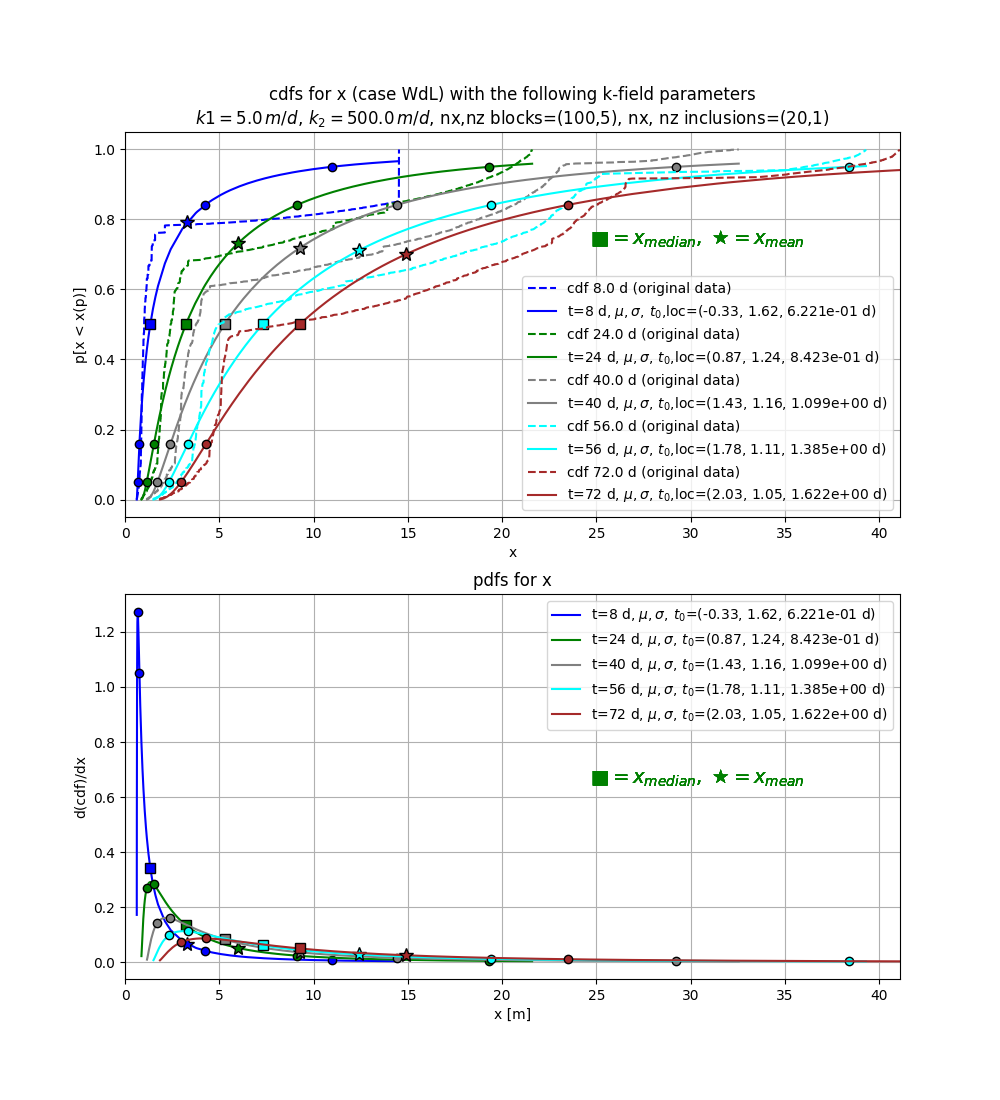
\includegraphics[width=0.8\textwidth]{/Users/Theo/GRWMODELS/python/mf6lab/Projects/Dispersion/cases/wimsaquif/images/BTanalysis_x_WdL}

\caption{\label{fig:wdl-BT-x}Top: Cumulative distribution of particles for
different times as a function of $x$. The fit is not very good for
this type of cross section, contrary to the break-through curves for
differetn $x$ as a function of time. The fitted pdfs clearly show
a large skew relative to those for the breakthrough at different values
of $x$ in the previous figure. Note that the traveled distance at
the observation times is really short compared to the length of the
cross section, while the particles that were captured at the different
observation locatons have all traveled a much larger distance through
the model.}

\end{figure}


\subsection{Test case}

It's important to run a test case that allows verification of the
procedures developed for this work. The chosen test case has the same
cross section of 100 rows and 1000 columns with cells of 1x1 m$^{2}$.
The aquifer is, therefore, 100 m thick and 1000 m long. The porosity
is kept the same as before. The fixed gradient of $J=0.0036$ was
maintained. The section was divided into 10 blocks each consisting
of 10 model layers. The conductivity is constant in each block and
increases in 10 steps from 1 m/d to 10 m/d. Hence, the first 10 model
layers all have $k=1$ m/d, the model layers 11 through 20 all have
$k=2$ m/d and so on until layers 91 through 100, which all have $k=100$
m/d. With this setup, the discharge through each layer and the travel
time in them as well as the location of each particle at any time
are now known and the model outcomes can now be verified by simple
hand calculculations.

The mean conductivity of this setup equals $k_{mean}=5.5$ m/d and
the total discharge $Q=k_{mean}\times D\times J=0.55\times100\times0.0036=1.98$
m$^{2}$/d. The Modflow listfile gives 1.98 m$^{2}$/d. The hand-computed
travel times are also essentially the same as the ones computed by
Modflow for all observation distances and for all layers. Finally
the hand-calculated positions of the particles at the chosen observation
times are essentially equal to the Modfpath calculated positions.

\begin{figure}[h]
\centering
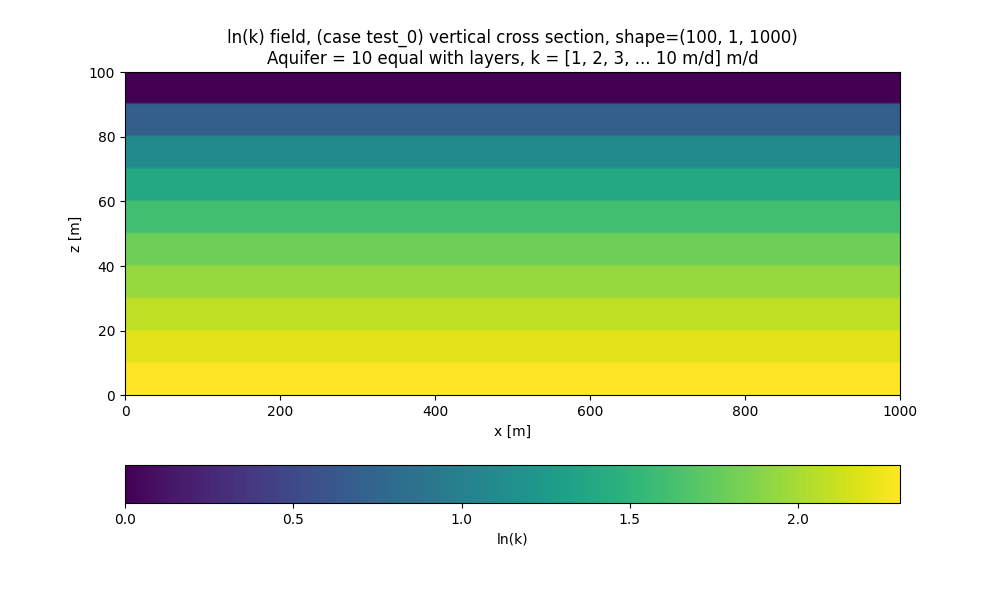
\includegraphics[width=0.8\textwidth]{/Users/Theo/GRWMODELS/python/mf6lab/Projects/Dispersion/cases/wimsaquif/images/kfield_test_0}

\caption{\label{fig:test0-kfield}Conductivity field of the test case.}

\end{figure}

\begin{figure}[h]
\centering
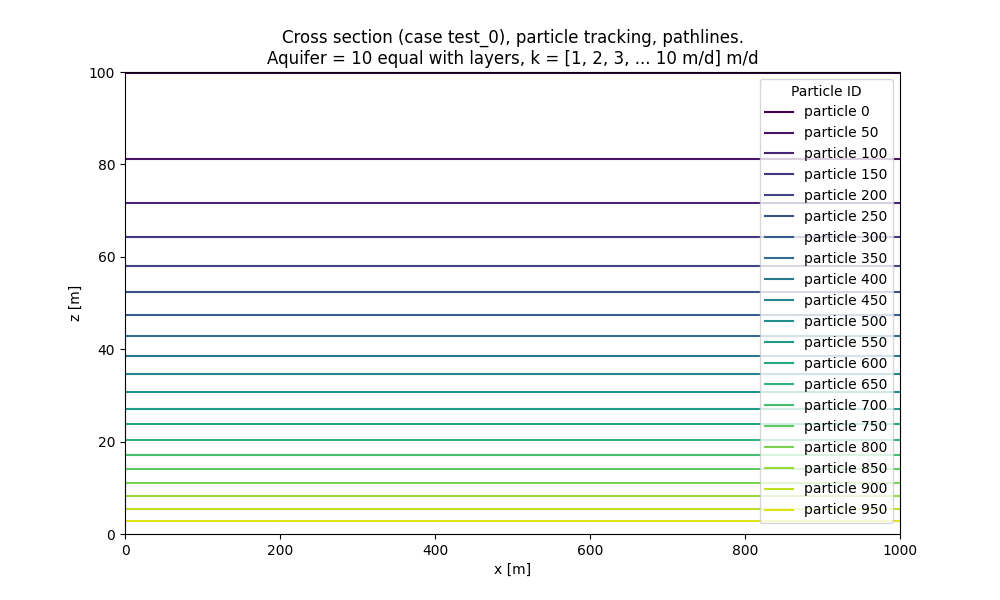
\includegraphics[width=0.8\textwidth]{/Users/Theo/GRWMODELS/python/mf6lab/Projects/Dispersion/cases/wimsaquif/images/plines_test_0}

\caption{\label{fig:test0-paths}Path lines test0. The difference in distance
between the path lines is because each path line represents the same
fraction of the total discharge through the cross section.}

\end{figure}

\begin{figure}[h]
\centering
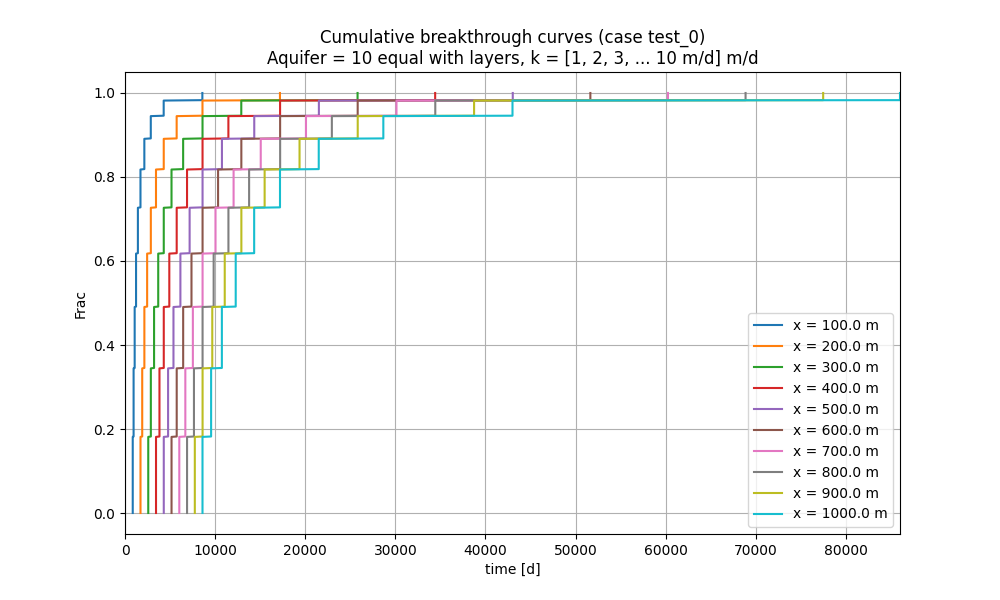
\includegraphics[width=0.8\textwidth]{/Users/Theo/GRWMODELS/python/mf6lab/Projects/Dispersion/cases/wimsaquif/images/cumul_t_test_0}

\caption{\label{fig:test0-cum-t}Break-through curves}

\end{figure}

\begin{figure}[h]
\centering
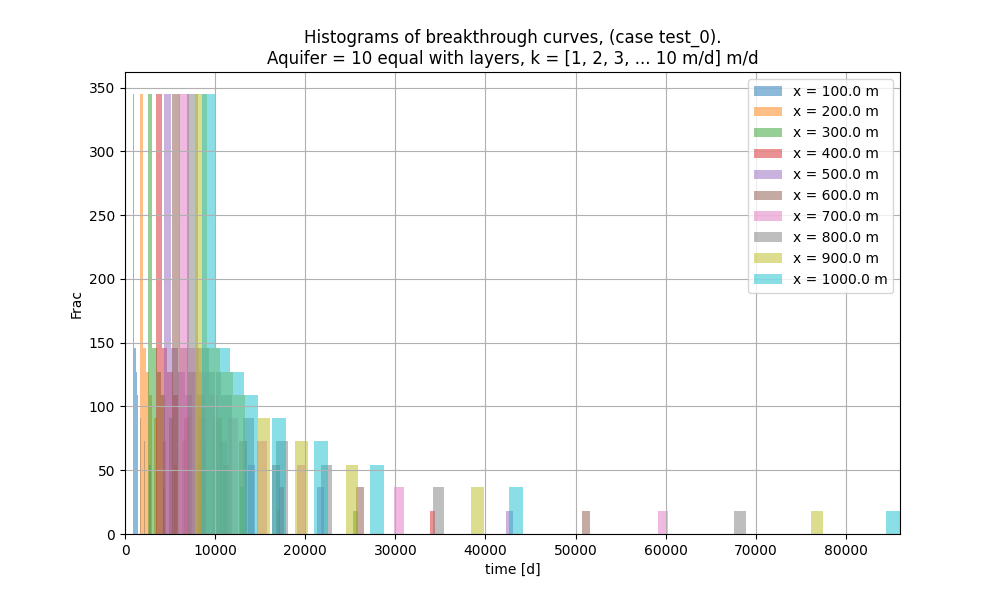
\includegraphics[width=0.6\textwidth]{/Users/Theo/GRWMODELS/python/mf6lab/Projects/Dispersion/cases/wimsaquif/images/hist_t_test_0}

\caption{\label{fig:test0-hist-t}Histograms for breakthrough times}

\end{figure}

\begin{figure}[h]
\centering
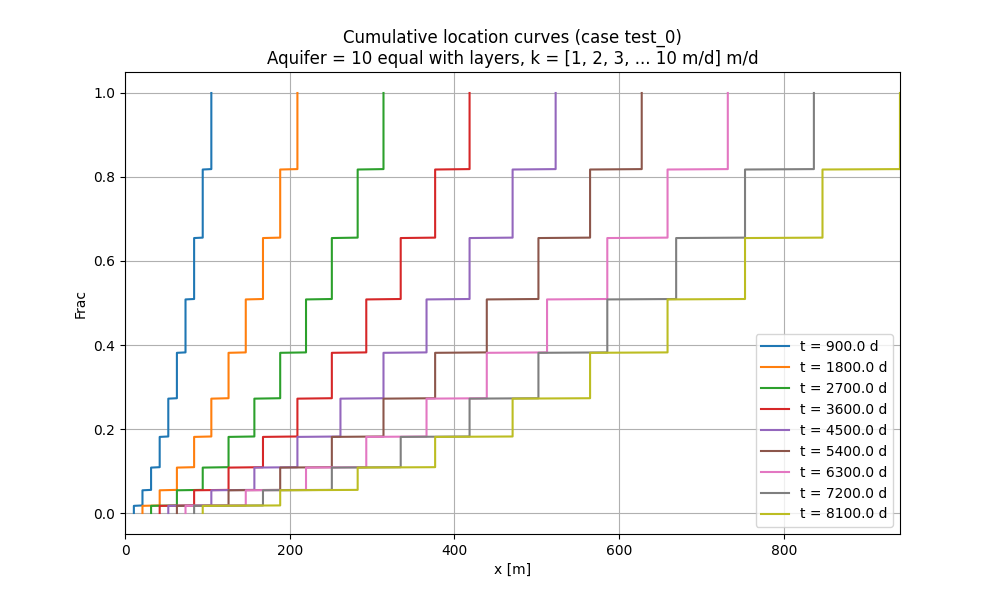
\includegraphics[width=0.8\textwidth]{/Users/Theo/GRWMODELS/python/mf6lab/Projects/Dispersion/cases/wimsaquif/images/cumul_x_test_0}

\caption{\label{fig:test0-cum-x}Cumulative location curves.}

\end{figure}

\begin{figure}[h]
\centering
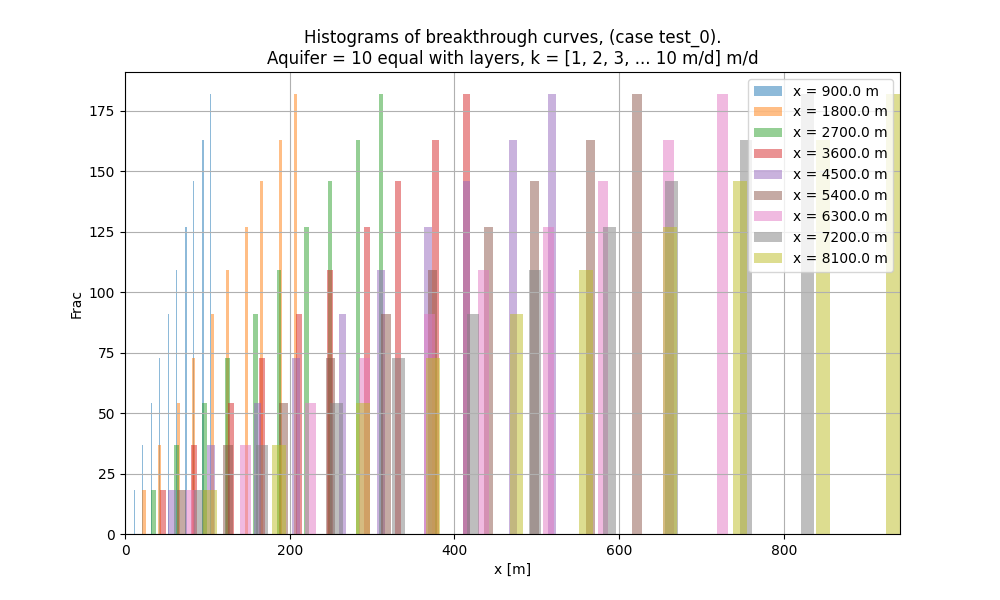
\includegraphics[width=0.8\textwidth]{/Users/Theo/GRWMODELS/python/mf6lab/Projects/Dispersion/cases/wimsaquif/images/hist_x_test_0}

\caption{\label{fig:test0-hist-x}}

\end{figure}

\begin{figure}[h]
\centering
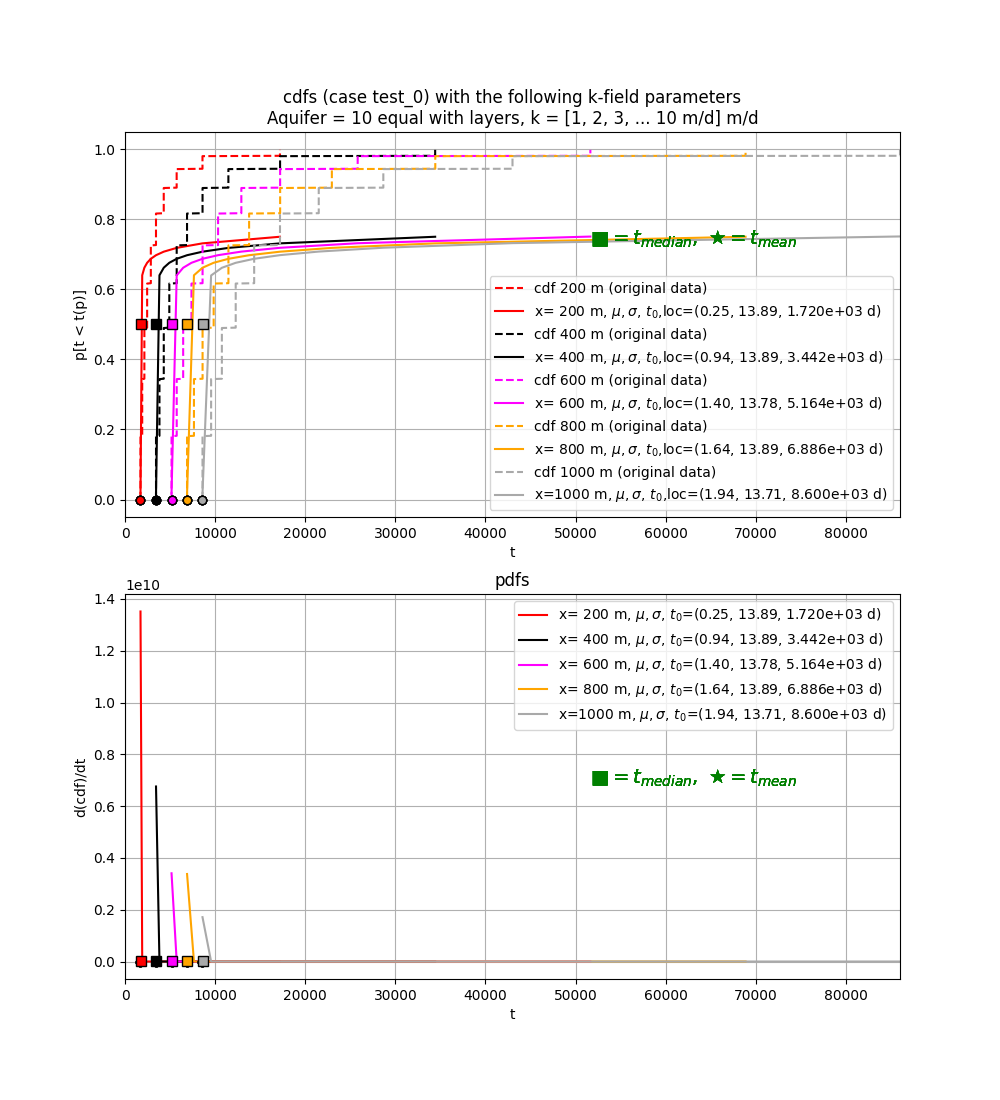
\includegraphics[width=0.8\textwidth]{/Users/Theo/GRWMODELS/python/mf6lab/Projects/Dispersion/cases/wimsaquif/images/BTanalysis_t_test_0}

\caption{\label{fig:test0-BT-t}Fitted cdfs and their pdfs. Fit fails with
this data (data that is essentially not random)}

\end{figure}

\begin{figure}[h]
\centering
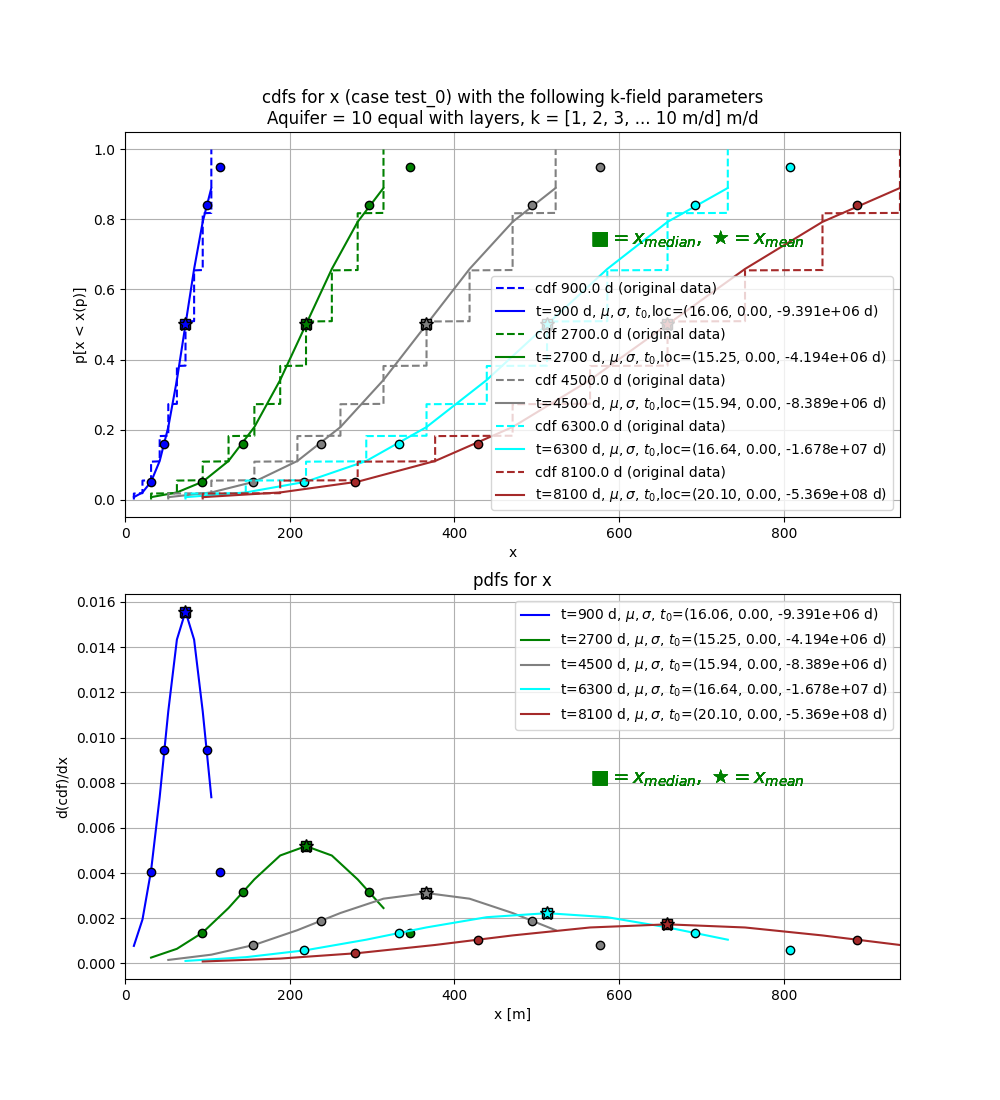
\includegraphics[width=0.8\textwidth]{/Users/Theo/GRWMODELS/python/mf6lab/Projects/Dispersion/cases/wimsaquif/images/BTanalysis_x_test_0}

\caption{\label{fig:test0-BT-x}Fitted location curves. Works but is useless
with this non-random test case.}

\end{figure}


\section{Summarizing the discussion on dispersion}

A phenomenon, including that of dispersion of a pollutant in moving
groundwater, can often be best understood by looking at its behavior
or results in extreme situations. We may, therefore, ask ourselves
how dispersion develops in the following two extreme cases:
\begin{itemize}
\item Uniform flow in a perfectly homogenious aquifer, with grains as fine
as the water molucules themselves. Hence, there are no velocity variations.
\item Flow in an aquifer that is layered and heterogeneous to the extreme.
Hence, it consists of two parallel layers one with (almost) zero conductivity
and the other with some distinct conductivity.
\end{itemize}
Over these cases, we may drape the process of diffusion, which is
known to always work and does so at its own pace, irrespective of
the actual velocity of the groundwater itself.

In the first case, the only movement of particles is the progress
of the front, initally flat and pependicular to the flow, which will
always remain sharp and stay perfectly flat. The only thing diffusion
does is to cause some spread in longitudinal direction. Without diffusion,
the breakthrough curve would be vertical. With diffusion it would
still be very steep. The breakthrough curve would be fully described
by the average front position and its standard deviation $\sigma=\sqrt{2D_{d}t}$.
Even if the particles would be subject to some small-scale random
velocity varations, the front will have the same properties, with
a $\sigma$ that will be larger than that caused by molecular diffusion,
probably even be much larger, but would still follow this expression
$\sigma=\sqrt{2Dt}$. Only now we have $D=D_{v}+D_{d}$ and since
the random velocity differences are proportional to the groundwater
velocity itself, we would have $D=a_{L}v+D_{d}$ and the process would
be fully Gaussian and Fickian, with a head and tail of the same length
and shape.

In the second extreme case, a part, may be half of the water will
be funelled through the high-conductive layer, with the rest lagging
far behind. When we call the situation at some point in time also
a plume, we see that we have a head and a tail completely defined
by the velocities in the two layers. Let the velocity in the two layers
be $v_{1}$ and $v_{2}$ with conductivities $k_{1}$ and $k_{2}$
respectively and a gradient $i$ and porosity $\theta$, we have

\begin{align*}
v_{1} & =k_{1}i/\theta\\
v_{2} & =k_{2}i\theta
\end{align*}

The total discharge through the aquifer then equals

\[
Q\theta=D_{1}k_{1}i+D_{2}k_{2}i=Dk_{m}i
\]

With $D_{1}$ and $D_{2}$ the thicknesse of the respective zones
and $D$ the aquifer thickness.

Assume that the same amoun of water flows through both zones, so that
$D_{1}k_{1}=D_{2}k_{2}$

\begin{align*}
k_{m} & =2\frac{D_{1}}{D}k_{1}\\
k_{m} & =2\frac{D_{2}}{D}k_{2}
\end{align*}

We are still free to choose $k_{1}/k_{2}$ or $D_{1}/D_{2}$ or $D_{1}/D$
for that matter. Just take $D_{1}=0.1D_{2}$so that $k_{1}=10k_{2}$
then 

\begin{align*}
k_{m} & =2\frac{0.1}{1.1}k_{1}\approx0.19k_{1}\rightarrow k_{1}\approx5.3k_{m}\\
k_{m} & =2\frac{0.9}{1.1}k_{2}\approx1.64k_{2}\rightarrow k_{2}\approx0.61k_{m}
\end{align*}

We could even take a more extreme case in which $D_{1}=0.001D_{2}$
so that $k_{1}=1000k_{2}$ yielding 

\[
k_{m}=2\frac{0.001}{1.001}k_{1}=2\frac{0.999}{1.001}k_{2}\approx0.002k_{1}\approx2k_{2}
\]

in which still half of the discharge flows through the thin conductive
layer and the other half through the thick layer with the lower conductivity.
In these, cases, even when equal amounts of water pass through both
zones, the distance traveled in the fast, high-conductive zone is
more than 5 to 500 times the average traveled distance, and that in
the low-conductive zone is about 60\% to 50\% of the average traveled
distance, where 50\% is the limit case.

What happens if we sample the water by means of a well that extracts
all the water at a certain point? Then, as soon as the fast front
passed this point, the relative concentration would jump to 0.5 to
remain constant until the tail passes, at which point the relative
concentration would jump further to 1.0. From these samples one could
conclude that the mean of the front would lie half way between the
two mentioned times and that its spread would amount to $\sigma=\frac{t_{1}-t_{2}}{\sqrt{2}}$.
On the other hand, if one samples the aquifer without actually extracting
water by a well, for instance by means of a device that can measure
some quality aspect in situ at any depth, and if we then take the
mean along the vertical, a completely different breakthrough curve
would emerge. As the fast zone has only one tenth or even one thousandth
of the thickness of that of the slow zone, the relative concentration
would, after passing the sampling location, only jump up to 0.1 or
to 0.001 instead of 0.5 and would rise to 1. 0 after passage of the
front in the slow zone. Therefore, the way of sampling may make a
huge difference in the outcomes.

What also jumps into mind in this extreme case, is that the spread,
i.e. the distance between head and tail, grows proportionally to time
and, therfore with distance. In the case of Fickian disperion it grows
proportional to the root of time. Reality will likely pop up somewhere
in between.

If we drape diffusion or our ignored random small-scale velocity velocity
variations over the last situation, there will be some longitudinal
dispersion, which may be negligible relative to the fast moving head
of the front. However, we will also see some dispersion across the
horziontal line separting the two zones. The importance of this sideways
spreading depends on the magnitude of the process, or perhaps to the
absolute speed of the groundwater relative to diffusion. Nevertheless,
if one imagines a very large sideways dispersion, it would cause the
head of the front to loose concentration to the water in the slow
zone. The larger this process the more the end result will resemble
Fickian behavior. Imagine that the fast zone were split into a vast
number of subzones spread out over the vertical but still making sure
that the combined transmissivity of these fast subzones remains equal
to that of the original one. This would make diffusion dominant instead
of negligible, even with the same overal transmissivities, conductivities
and zone thicknesses; it would completely alter the shape of the front.
Hence, size or layering matters. This includes time as it affects
the size of the spread by diffusion, which, as we have seen will grow
to aquifer-height proportions if sufficiently long. Even much shorter
times may be important if the fast and the slow layers are thin. Reality
will always be somewhere in between. The more homogeneous the aquifer,
or the thinner the layers, the more Fickian the dispersion process
will be. The more heterogeneous in the sense that the flow is more
dominated by preferential flow paths, the less Fickian the dispersion
will be, and the more its spread with grow linearly with time and
distance. Because the streamlines in real-world cases will pass through
sequences of zones of higher and lower conductivties of different
extent, the spread may grow towards linear with traveled distance,
the larger the probability of encountering high-conductivity zones
of even larger exent that channel the grounwater along preferential
paths.

\section{Summary and conclusions}

Dispersion during subsurfacde mass transpport was studied based on
recent papers as mentioned in the references. The phenomemon of dispersion
is still not totally tackeled in models as well as in theory. \cite{Zheng11}
mentioned the dual medium feature, adding kinematic sorption, that
was built into the MT3DMS mass transport model to better capture the
observations of tracer tests in the Made test side \cite{Zheng11}.
However, the improved match may well have been reached for the wrong
reasons, as there was no sorption active at the site during the bromium
tracer test. At least \cite{Fiori13} showed that a similarly accurate
result could be reached with their MIM (multi indicator model), which
only took advection into account. The problem is believed to has been
the impossibility to characterize and model the heterogeneous conductivity
field in the subsurface accurately enough, because therein seems to
lie the key to successfully model subsurface displacement of pollutants
and successfully include match the observed dispersion.

It is generally known that in real-world situations flow along preferential
paths is often dominant. At the same time, it is extremely hard to
predict beforehand based on methods available to characterize the
subsruface's conductivity field in all three dimensions. While in
more homogeneous aquifers dispersion tends toward Fickian behavior,
in heterogeneous aquifers it does not. Fickian behavior sees dispersion
as a Gaussian process, which yields symmetrical breakthrough curves
and histograms with the spread that grows according to the square
root of the traveled distance. However, non Fickian behavior as observed
in hetrogeneous aquifers, show asymmetrical breakhrough curves and
histograms, with early breakthorugh and a large tail, with an associated
spread that grows linearly with travel distance.

This non-Fickian behavior was shown by modelling a heterogeneous aquifer
with the properties of the Made site (\cite{Fiori13}). The aquifer
generated with those parameter values, was similar to that by which
\cite{Fiori13} were able to reasonably well model the bromide tracer
test at the Made site. The results show indeed that the breaktrough
curves and breakthrough histograms have an early breakthrough with
a long tail. The opposite, more Fickian result was obtained by modeling
another cross section generated with the same parameters, but with
a far lower $\ln\left(k\right)$ variance, which resulted in a much
more homogeneous aquifer. The aquifer used by \cite{Fiori13} consisted
of blocks with a length of around 20 m based on the horizontal integration
scale (range of the semi-variogram). Each block got a conductivity
value chosen from a generated random field with the proper statistical
values. In the third example, we left the block structure out and
directly used the statistically generated conductivity field. The
results show that they are similar to those of the first example,
generated with the same statistical parameter values (see the header
of each figure for the values used). Hence, using the block structure
does not seem to add much to the results; only the horizontal and
verticla semi-variograms used to generate the random field seem to
matter.

Finally, a cross section was generated alike the one De Lange uses
in his papers to demonstrate and simulate dispersion in very heterogeneous
aquifers. De Lange, for the sake of modelling dispersion, sees the
aquifer as layers of equally sized blocks called domains, which are
put next to and on top of each other to fill the aquifer. Each block
has a low background conductivity (of 5 m/d) and holds an elongated,
rectangular inclusion with a high conductivity (of 500 m/d). This
cross section was simulated in the same way as the previous ones.
Expected was a strong non-Fickian behavior to show up in the breakthrough
curves and the histograms. However, this proved hardly the case. So
perhaps the cross section was not heterogeneous enough, despite the
100-fold conductiviy contrast between the background and the included
facies conductivities.

\addcontentsline{toc}{section}{Referenties}

\section{Analysis of the lognormal distribution}

\[
\mathtt{if}\,T\sim LogNormal\left(\mu,\sigma\right)\rightarrow\log T\sim N\left(\mu,\sigma\right)
\]

When retrieving the lognormal distribution or generating it, it has
three parameters scale, loc, shape, where

$\mu=\ln\left(scale\right)$

$\sigma=shape$

$loc$=linear shift in the time domain (real world domain)

\[
t\sim LogNormal\left(\mu,\sigma,\mathtt{loc}\right)
\]

is equivalent to saying

\[
\ln\left(t-\mathtt{loc}\right)\sim N\left(\mu,\sigma^{2}\right)
\]

Or, rearranged

\[
t=\mathtt{loc}+\exp\left(X\right),\,\,\,\,X\sim N\left(\mu,\sigma^{2}\right)
\]

\begin{enumerate}
\item Hence, $\mathtt{loc}$ acts as a shift in the time domain.
\item It's the minimum value the variable $t$ can take -- the distribution
is defined for $t>\mathtt{loc}.$
\item It's ofteh use to delya th eonset of the lognormal process.
\end{enumerate}
Further properties of the lognormal distribution

\[
\mathtt{mean}\left(t\right)=\mathtt{loc}+\exp\left(\mu+\frac{\sigma^{2}}{2}\right)
\]

\[
\mathtt{median}\left(t\right)=\mathtt{loc}+\exp\left(\mu\right)
\]

\[
\mathtt{mode}\left(t\right)=\mathtt{loc}+\exp\left(\mu-\sigma^{2}\right)
\]

Head and tail quantiles may be useful, but more so in log-space than
in real-space due to the skewness of the lognormal distribution. The
quantile times s $t_{05}$, $t_{16}$, $t_{50}$, $t_{84}$ and $t_{95}$
can also easily obtained from a given cdf or pdf distribution, but
these too are less informative for the lognormal distribution than
for the normal distribution. 

\begin{table}[h]
\centering
\caption{Head and tail quantiles}

\begin{tabular}{|c|c|c|}
\hline 
Region & Log-space range & Time space rang\tabularnewline
\hline 
\hline 
Head & $\mu-2\sigma\,\mathtt{to}\,\mu-\sigma$  & $\left[e^{\mu-2\sigma},e^{\mu-\sigma}\right]$\tabularnewline
\hline 
Bulk & $\mu-\sigma\,\mathtt{to}\,\mu+\sigma$ & $\left[e^{\mu-\sigma},e^{\mu+\sigma}\right]$\tabularnewline
\hline 
Tail & $\mu+\sigma\,\mathtt{to}\,\mu+2\sigma$ & $\left[e^{\mu+\sigma},e^{\mu+2\sigma}\right]$\tabularnewline
\hline 
\end{tabular}

\end{table}

Let $x$ be the traveled distanc, then

\begin{table}[h]
\centering
\caption{Velocities}

\begin{tabular}{|c|c|c|}
\hline 
\begin{cellvarwidth}[t]
\centering
Time

statitic
\end{cellvarwidth} & Velocity=distance/time & Behavior\tabularnewline
\hline 
\hline 
Mean & $v_{\mathtt{mean}}=x/\left(\mathtt{loc}+\exp\left(\mu+\sigma^{2}/2\right)\right)$ & Roughly constant$\rightarrow$average advection\tabularnewline
\hline 
Mode & $v_{\mathtt{mode}}=x/\left(\mathtt{loc}+\exp\left(\mu-\sigma^{2}\right)\right)$ & \begin{cellvarwidth}[t]
\centering
Decreases with increasing x, since the distribution skews more.

Early arrivals shift right as distance increases (due to dispersion)
\end{cellvarwidth}\tabularnewline
\hline 
\end{tabular}
\end{table}

Physical interpretation:
\begin{itemize}
\item The mean reflects the center of mass of the particle plume.
\item The mode reflects the most probable arrival time, which is more sensitive
to early or delayed arrivals due to dispersion.
\item When the mean velocity remains constant confirms a linear advecton
front.
\item The the mode shifts sublinearly with distance implies that the spread
(dispersion) becomes more significant with distance, skewing the distributioin
more and pushing the peak back.
\item The median is the time at which the cdf=0.5 as half the particles
take shorter and the other half longer than this time.
\item The mean velocity is equal to the surface to the left of the cdf.
This too is obvious.
\item The model is the time at which the cdf is steepest, i.e. its first
derivative peaks (this is obviously the top of the pdf).
\end{itemize}
An easy and informative criterion for early and late arrivals may
be built on $\mathtt{loc}$ as the earlies possible moment of arrival
of particles and $t_{mode}$ as the most probable time of arrival.
We may select point based on the ratio of these two times. Let's,
just for convenience rename $\mathtt{loc}$

\[
t_{0}=\mathtt{loc}
\]

then we can base arrival time criteria on the ratio

\[
\alpha=\frac{t-t_{0}}{t_{mode}-t_{0}}
\]

and so

\[
t=t_{0}+\left(t_{mode}-t_{0}\right)\alpha
\]

and use the following arrival criteria

\begin{table}[h]
\centering

\caption{Arrival criteria}

\begin{tabular}{|c|c|}
\hline 
$\alpha$-range  & Arrival type\tabularnewline
\hline 
\hline 
$0.0\,-\,0.2$ & Very early arrivals\tabularnewline
\hline 
$0.2\,-\,0.5$ & Early arrivals\tabularnewline
\hline 
$0.5\,-\,2.0$ & Normal arrivals\tabularnewline
\hline 
$2.0\,-\,5.0$ & Late arrivals\tabularnewline
\hline 
$>5.0$ & Very late arrivals\tabularnewline
\hline 
\end{tabular}

\end{table}

\begin{thebibliography}{Hemker and Bakker (2004)}
\bibitem[Bowling et al. (2005)]{Bow05}Bowling, J.C., Rodirguez, A.B.,
Harray, D.L., Zheng, C. (2005) Deliniating Alluvial Aquifer Heterogeneity
Using Resistivity and GPR Data. Ground Water, Vol. 43, No. 6. p890-903.

\bibitem[Coe (2003)]{Coe03}Coe, AlL. (2003) The sedimentological
record of sea-level change. Cambridge Univeristy Press, Cambridge
UK. ISBN 0-521-53852-4. 279p.

\bibitem[Fiori et al. (2013)]{Fiori13}Fiori, A., Dagan, G., Jankovic,
I. \& Zarlenga, A (1213) The plume spreading in he Made transport
experiment: Could it be predicted by stochastiv models? WRR, Vol.
49, 1-11, doi:10.1002/wrcr.20128 2013.

\bibitem[Hemker and Bakker (2004)]{HemBak04}Hemker, C. J., Van den
Berg, E., \& Bakker, M. (2004). Ground water whirls. Ground Water,
42(2), 234--242.

\bibitem[De Lange (2025)]{Lange25}Lange, W.J. de (2025) Using Advective
Transport Phenomena In Modeling To Better Understand Mechanical Dispersion:
Step One. In preparation.

\bibitem[De Lange (2022)]{Lange22}Lange, W.J. de (2022) Advective
Transport Phenomena to Better Understand Dispersion in Field and Modeling
Practice. Groundwater 58, 46--55. https://doi.org/10.1111/gwat.12883

\bibitem[De Lange (2020)]{Lange20}Lange, W.J. de (2020) Advective
Transport Phenomena to Better Understand Dispersion in Field and Modeling
Practice. Groundwater 58, 46--55. https://doi.org/10.1111/gwat.12883

\bibitem[Jankovic et al. (2010)]{Jankovic10}Janković, I., \& Fiori,
A. (2010). Anomalous transport in highly heterogeneous 3D aquifers:
A numerical study. Water Resources Research, 46(10), W10502. https://doi.org/10.1029/2009WR008839

\bibitem[Jankovic et al. (2006)]{Jankovic06}Jankovic, I, Fiori, A,
\& D. Dagan (2006) Modeling flow and transport in highly heterogeneous
three-dimensional aquifers: Ergodicity, Gaussianity, and anomalous
behavior. I Conceptual issues and numerical simulations. WRR, Vol.42,
W06D12, doi:10.1029/2005/WR004734. 9p.

\bibitem[Jankovic et al. (2003)]{Jankovic03}Janković, I., Fiori,
A., \& Dagan, G. (2003). Flow and transport in highly heterogeneous
formations: 3D numerical simulations and the validity of the Boussinesq
approximation. Water Resources Research, 39(3), 1045. https://doi.org/10.1029/2001WR001182\LyXZeroWidthSpace{}

\bibitem[Sudicky (1986)]{Sudicky86}Sudicky EA (1986) A Natural Gradient
Experiment on Solute Transport in a Sand Aquifer: Spatial Variability
of Hydraulic Conductivity and Its Role in the Dispersion Process.
WRR 22(1986)13, 2069-2082.

\bibitem[Zheng et al. (2011)]{Zheng11} Zheng, C., Bianhi, M. \& Corelick
S.M. (2011) Lessons Learned from 25 Years of Research. Review paper.
Ground Water, 29(5), 649-662. https://doi.org/10.1111/j.1745-6584.2010.00753.x\&\#8203

\bibitem[Jensen et al. (1993)]{Jensen93}Jensen K. Hogh \& Bitsh K.
(1993) Large-scale Dispersion Experiments in a Sandy Aqufier in Denmark:
Observed Tracer Movements and Numerical Analysis. WRR Vol.29, No.
3, 673-696

\end{thebibliography}


\end{document}
